% Options for packages loaded elsewhere
\PassOptionsToPackage{unicode}{hyperref}
\PassOptionsToPackage{hyphens}{url}
\PassOptionsToPackage{dvipsnames,svgnames,x11names}{xcolor}
\documentclass[
  10pt,
  fontset=fandol]{ctexart}
\usepackage{xcolor}
\usepackage[margin=16mm]{geometry}
\usepackage{amsmath,amssymb}
\setcounter{secnumdepth}{-\maxdimen} % remove section numbering
\usepackage{iftex}
\ifPDFTeX
  \usepackage[T1]{fontenc}
  \usepackage[utf8]{inputenc}
  \usepackage{textcomp} % provide euro and other symbols
\else % if luatex or xetex
  \usepackage{unicode-math} % this also loads fontspec
  \defaultfontfeatures{Scale=MatchLowercase}
  \defaultfontfeatures[\rmfamily]{Ligatures=TeX,Scale=1}
\fi
\usepackage{lmodern}
\ifPDFTeX\else
  % xetex/luatex font selection
\fi
% Use upquote if available, for straight quotes in verbatim environments
\IfFileExists{upquote.sty}{\usepackage{upquote}}{}
\IfFileExists{microtype.sty}{% use microtype if available
  \usepackage[]{microtype}
  \UseMicrotypeSet[protrusion]{basicmath} % disable protrusion for tt fonts
}{}
\makeatletter
\@ifundefined{KOMAClassName}{% if non-KOMA class
  \IfFileExists{parskip.sty}{%
    \usepackage{parskip}
  }{% else
    \setlength{\parindent}{0pt}
    \setlength{\parskip}{6pt plus 2pt minus 1pt}}
}{% if KOMA class
  \KOMAoptions{parskip=half}}
\makeatother
\usepackage{longtable,booktabs,array}
\newcounter{none} % for unnumbered tables
\usepackage{calc} % for calculating minipage widths
% Correct order of tables after \paragraph or \subparagraph
\usepackage{etoolbox}
\makeatletter
\patchcmd\longtable{\par}{\if@noskipsec\mbox{}\fi\par}{}{}
\makeatother
% Allow footnotes in longtable head/foot
\IfFileExists{footnotehyper.sty}{\usepackage{footnotehyper}}{\usepackage{footnote}}
\makesavenoteenv{longtable}
\usepackage{graphicx}
\makeatletter
\newsavebox\pandoc@box
\newcommand*\pandocbounded[1]{% scales image to fit in text height/width
  \sbox\pandoc@box{#1}%
  \Gscale@div\@tempa{\textheight}{\dimexpr\ht\pandoc@box+\dp\pandoc@box\relax}%
  \Gscale@div\@tempb{\linewidth}{\wd\pandoc@box}%
  \ifdim\@tempb\p@<\@tempa\p@\let\@tempa\@tempb\fi% select the smaller of both
  \ifdim\@tempa\p@<\p@\scalebox{\@tempa}{\usebox\pandoc@box}%
  \else\usebox{\pandoc@box}%
  \fi%
}
% Set default figure placement to htbp
\def\fps@figure{htbp}
\makeatother
\setlength{\emergencystretch}{3em} % prevent overfull lines
\providecommand{\tightlist}{%
  \setlength{\itemsep}{0pt}\setlength{\parskip}{0pt}}
\usepackage{amsmath,amssymb,mathtools,needspace}
\xeCJKDeclareCharClass{CJK}{"2032,"0400->"04FF,"2160->"216B,"2460->"2473,"25A0,"25C7,"25CB,"25CF}
\IfFontExistsTF{Arial Unicode MS}{\xeCJKsetup{AutoFallBack=true}\setCJKfallbackfamilyfont{\CJKrmdefault}{Arial Unicode MS}}{}
\setcounter{secnumdepth}{0}
\setlength{\emergencystretch}{2em}
\allowdisplaybreaks
\usepackage{bookmark}
\IfFileExists{xurl.sty}{\usepackage{xurl}}{} % add URL line breaks if available
\urlstyle{same}
\hypersetup{
  pdftitle={常微分方程数值解法},
  colorlinks=true,
  linkcolor={Maroon},
  filecolor={Maroon},
  citecolor={Blue},
  urlcolor={Blue},
  pdfcreator={LaTeX via pandoc}}

\title{常微分方程数值解法}
\author{}
\date{}

\begin{document}
\maketitle

\section{第 5 章 常微分方程数值解法}\label{ux7b2c-5-ux7ae0-ux5e38ux5faeux5206ux65b9ux7a0bux6570ux503cux89e3ux6cd5}

\subsection{5.1 引言}\label{ux5f15ux8a00}

科学技术中常常需要求解常微分方程的定解问题。这类问题最简单的形式，是本章将要着重考察的一阶方程的初值问题

\[
y'=f(x,y),\tag{5.1.1}
\]

\[
y(x_0)=y_0.\tag{5.1.2}
\]

我们知道，只要函数 \(f(x,y)\) 适当光滑------譬如关于 \(y\) 满足 Lipschitz 条件

\[
|f(x,y)-f(x,\bar y)|\leqslant L|y-\bar y|,
\]

理论上就可以保证初值问题 (5.1.1)、(5.1.2) 的解 \(y=y(x)\) 存在并且唯一。

虽然求解常微分方程有各种各样的解析方法，但解析方法只能用来求解一些特殊类型的方程，实际问题中归结出来的微分方程主要靠数值解法求解。

所谓\textbf{数值解法}，就是寻求解 \(y(x)\) 在一系列离散节点

\[
x_1<x_2<\cdots<x_n<x_{n+1}<\cdots
\]

上的近似值 \(y_1,\allowbreak y_2,\allowbreak \cdots,\allowbreak y_n,\allowbreak y_{n+1},\allowbreak \cdots\)。相邻两个节点的间距 \(h=x_{n+1}-x_n\) 称为\textbf{步长}。今后如不特别说明，总是假定 \(h\) 为定数，这时节点为 \(x_n=x_0+nh\)，\(n=0,1,2,\cdots\)。

初值问题 (5.1.1)、(5.1.2) 的数值解法有个基本特点，它们都采取``步进式''，即求解过程顺着节点排列的次序一步一步地向前推进。描述这类算法，只要给出用已知信息 \(y_n,y_{n-1},y_{n-2},\cdots\) 计算 \(y_{n+1}\) 的递推公式即可。这种计算公式称为\textbf{差分格式}。

\subsection{5.2 Euler 方法}\label{euler-ux65b9ux6cd5}

\subsubsection{5.2.1 Euler 格式}\label{euler-ux683cux5f0f}

我们知道，在 \(Oxy\) 平面上，微分方程 (5.1.1) 的解 \(y=y(x)\) 称为它的\textbf{积分曲线}。积分曲线上一点 \((x,y)\) 的切线斜率等于函数 \(f(x,y)\) 的值。如果按函数 \(f(x,y)\) 在 \(Oxy\) 平面上建立一个方向场，那么，积分曲线上每一点的切线方向均与方向场在该点的方向一致。

基于上述几何解释，我们从初始点 \(P_0(x_0,y_0)\) 出发，先依方向场在该点的方向推

\href{../../source-images/pdf-120.jpeg}{原页}

进到 \(x=x_1\) 上一点 \(P_1\)，然后再从 \(P_1\) 依方向场的方向推进到 \(x=x_2\) 上一点 \(P_2\)，循此前进作出一条折线 \(P_0P_1P_2\cdots\)（见图 5.1）。

一般地，设已作出该折线的极点 \(P_n\)，过 \(P_n(x_n,y_n)\) 依方向场的方向再推进到 \(P_{n+1}(x_{n+1},y_{n+1})\)，显然两个极点 \(P_n,P_{n+1}\) 的坐标有下列关系：

\[
\frac{y_{n+1}-y_n}{x_{n+1}-x_n}=f(x_n,y_n),
\]

即

\[
y_{n+1}=y_n+hf(x_n,y_n).\tag{5.2.1}
\]

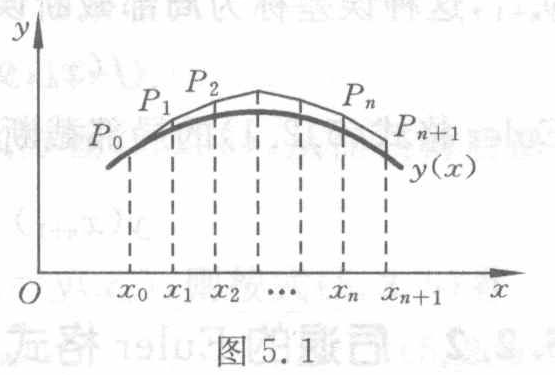
\includegraphics[width=0.85\linewidth,height=\textheight,keepaspectratio,alt={图 5.1 原图}]{../assets/ch05a/fig-5.1.png}

图 5.1（原图）：Euler 折线 \(P_0P_1P_2\cdots P_nP_{n+1}\) 与积分曲线 \(y(x)\)。原图符号标签：\(O,\allowbreak x,\allowbreak y,\allowbreak x_0,\allowbreak x_1,\allowbreak x_2,\allowbreak \cdots,\allowbreak x_n,\allowbreak x_{n+1},\allowbreak P_0,\allowbreak P_1,\allowbreak P_2,\allowbreak P_n,\allowbreak P_{n+1},\allowbreak y(x)\)。

这就是著名的 \textbf{Euler 格式}。若初值 \(y_0\) 已知，则依格式 (5.2.1) 可逐步算出

\[
y_1=y_0+hf(x_0,y_0),\qquad y_2=y_1+hf(x_1,y_1),\qquad\cdots.
\]

\textbf{例 5.1} 求解初值问题

\[
\begin{cases}
y'=y-2x/y\quad(0<x<1),\\
y(0)=1.
\end{cases}\tag{5.2.2}
\]

\textbf{解} 为便于比较，本章将用多种数值方法求解上述初值问题。这里先用 Euler 方法，Euler 格式的具体形式为

\[
y_{n+1}=y_n+h\left(y_n-\frac{2x_n}{y_n}\right).
\]

取步长 \(h=0.1\)，计算结果如表 5.1 所示。

\textbf{表 5.1}

{\def\LTcaptype{none} % do not increment counter
\begin{longtable}[]{@{}llllll@{}}
\toprule\noalign{}
\(x_n\) & \(y_n\) & \(y(x_n)\) & \(x_n\) & \(y_n\) & \(y(x_n)\) \\
\midrule\noalign{}
\endhead
\bottomrule\noalign{}
\endlastfoot
0.1 & 1.1000 & 1.0954 & 0.6 & 1.5090 & 1.4832 \\
0.2 & 1.1918 & 1.1832 & 0.7 & 1.5803 & 1.5492 \\
0.3 & 1.2774 & 1.2649 & 0.8 & 1.6498 & 1.6125 \\
0.4 & 1.3582 & 1.3416 & 0.9 & 1.7178 & 1.6733 \\
0.5 & 1.4351 & 1.4142 & 1.0 & 1.7848 & 1.7321 \\
\end{longtable}
}

初值问题 (5.2.2) 有解 \(y=\sqrt{1+2x}\)，按这个解析式子算出的准确值 \(y(x_n)\) 同近似值 \(y_n\) 一起列在表 5.1 中，二者相比较可以看出，Euler 方法的精度很差。

还可以通过几何直观来考察 Euler 方法的精度。假设 \(y_n=y(x_n)\)，即顶点 \(P_n\) 落在积分曲线 \(y=y(x)\) 上，那么，按 Euler 方法作出的折线 \(P_nP_{n+1}\) 便是 \(y=y(x)\) 过点 \(P_n\) 的切线（见图 5.2）。从图形上看，这样定出的顶点 \(P_{n+1}\) 显著地偏离了原来的积分曲线，可见 Euler 方法是相当粗糙的。

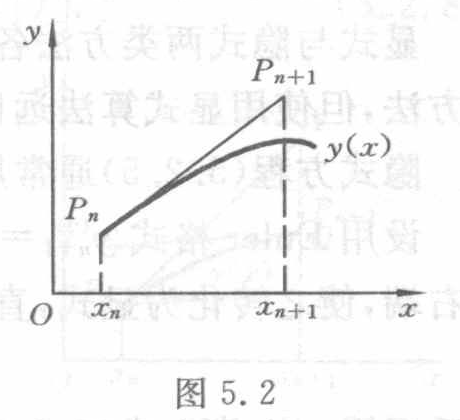
\includegraphics[width=0.85\linewidth,height=\textheight,keepaspectratio,alt={图 5.2 原图}]{../assets/ch05a/fig-5.2.png}

图 5.2（原图）：从积分曲线上 \(P_n\) 沿切线得到 \(P_{n+1}\)，与曲线 \(y(x)\) 在 \(x_{n+1}\) 的值有偏差。原图符号标签：\(O,\allowbreak x,\allowbreak y,\allowbreak x_n,\allowbreak x_{n+1},\allowbreak P_n,\allowbreak P_{n+1},\allowbreak y(x)\)。

人们常以 Taylor 展开为工具来分析计算公式的

\href{../../source-images/pdf-121.jpeg}{原页}

精度。为简化分析，假定 \(y_n\) 是准确的，即在 \(y_n=y(x_n)\) 的前提下估计误差 \(y(x_{n+1})-y_{n+1}\)，这种误差称为\textbf{局部截断误差}。注意到

\[
f(x_n,y_n)=f(x_n,y(x_n))=y'(x_n),
\]

Euler 格式 (5.2.1) 的局部截断误差显然为

\[
y(x_{n+1})-y_{n+1}=\frac{h^2}{2}y''(\xi)\approx\frac{h^2}{2}y''(x_n).\tag{5.2.3}
\]

\subsubsection{5.2.2 后退的 Euler 格式}\label{ux540eux9000ux7684-euler-ux683cux5f0f}

方程 \(y'=f(x,y)\) 中含有导数项 \(y'(x)\)，这是微分方程的本质特征，也正是它难以求解的症结所在。数值解法的关键在于设法消除其导数项，这项手续称为\textbf{离散化}。由于差分是微分的近似运算，实现离散化的基本途径之一是直接用差商替代导数。譬如，若在点 \(x_n\) 列出方程

\[
y'(x_n)=f(x_n,y(x_n)),\tag{5.2.4}
\]

并用差商 \(\dfrac{y(x_{n+1})-y(x_n)}{h}\) 近似替代其中的导数 \(y'(x_n)\)，结果有

\[
y(x_{n+1})\approx y(x_n)+hf(x_n,y(x_n)).
\]

设 \(y(x_n)\) 的近似值 \(y_n\) 已知，用它代入上式右端进行计算，并取计算结果 \(y_{n+1}\) 作为 \(y(x_{n+1})\) 的近似值，这就是 Euler 格式。

对于在点 \(x_{n+1}\) 列出的方程 (5.1.1)，有

\[
y'(x_{n+1})=f(x_{n+1},y(x_{n+1})),
\]

若用向后差商 \(\dfrac{y(x_{n+1})-y(x_n)}{h}\) 替代导数 \(y'(x_{n+1})\)，则可将上式离散化得

\[
\frac{y_{n+1}-y_n}{h}=f(x_{n+1},y_{n+1}),
\]

即

\[
y_{n+1}=y_n+hf(x_{n+1},y_{n+1}),\tag{5.2.5}
\]

此为\textbf{后退的 Euler 格式}。

后退的 Euler 格式与 Euler 格式有着本质的区别，后者是关于 \(y_{n+1}\) 的一个直接的计算格式，这类格式是\textbf{显式的}；而格式 (5.2.5) 的右端含有未知的 \(y_{n+1}\)，它实际上是关于 \(y_{n+1}\) 的一个函数方程，这类格式是\textbf{隐式的}。

显式与隐式两类方法各有特点。考虑到数值稳定性等因素，人们有时需要选用隐式方法，但使用显式算法远比隐式方便。

隐式方程 (5.2.5) 通常用迭代法求解，而迭代过程的实质是逐步显式化。

设用 Euler 格式 \(y_{n+1}^{(0)}=y_n+hf(x_n,y_n)\) 给出迭代初值 \(y_{n+1}^{(0)}\)，用它代入式 (5.2.5) 的右端，使之转化为显式，直接计算得

\[
y_{n+1}^{(1)}=y_n+hf(x_{n+1},y_{n+1}^{(0)}),
\]

然后再用 \(y_{n+1}^{(1)}\) 代入式 (5.2.5) 的右端，又有

\href{../../source-images/pdf-122.jpeg}{原页}

\[
y_{n+1}^{(2)}=y_n+hf(x_{n+1},y_{n+1}^{(1)}).
\]

如此反复进行迭代，得

\[
y_{n+1}^{(k+1)}=y_n+hf(x_{n+1},y_{n+1}^{(k)})\qquad(k=0,1,\cdots).
\]

如果迭代过程收敛，则极限值 \(y_{n+1}=\lim\limits_{k\to\infty}y_{n+1}^{(k)}\) 必满足隐式方程 (5.2.5)，从而获得后退的 Euler 方法的解。

再考察后退的 Euler 格式的局部截断误差。假设 \(y_n=y(x_n)\)，则按式 (5.2.5) 有

\[
y_{n+1}=y(x_n)+hf(x_{n+1},y_{n+1}),\tag{5.2.6}
\]

由于

\[
f(x_{n+1},y_{n+1})=f(x_{n+1},y(x_{n+1}))+f_y(x_{n+1},\eta)[y_{n+1}-y(x_{n+1})],
\]

其中 \(\eta\) 介于 \(y_{n+1}\) 与 \(y(x_{n+1})\) 之间。又

\[
f(x_{n+1},y(x_{n+1}))=y'(x_{n+1})=y'(x_n)+hy''(x_n)+\cdots,
\]

代入式 (5.2.6) 有

\[
y_{n+1}=hf_y(x_{n+1},\eta)[y_{n+1}-y(x_{n+1})]+y(x_n)+hy'(x_n)+h^2y''(x_n)+\cdots,
\]

将它与 Taylor 展开式

\[
y(x_{n+1})=y(x_n)+hy'(x_n)+\frac{h^2}{2}y''(x_n)+\cdots
\]

相减，得

\[
y(x_{n+1})-y_{n+1}=hf_y(x_{n+1},\eta)[y(x_{n+1})-y_{n+1}]-\frac{h^2}{2}y''(x_n)+\cdots.
\]

再注意到

\[
\frac{1}{1-hf_y(x_{n+1},\eta)}=1+hf_y(x_{n+1},\eta)+\cdots,
\]

最后整理，得

\[
y(x_{n+1})-y_{n+1}\approx-\frac{h^2}{2}y''(x_n).\tag{5.2.7}
\]

\subsubsection{5.2.3 梯形格式}\label{ux68afux5f62ux683cux5f0f}

比较 Euler 格式与后退的 Euler 格式的误差公式 (5.2.3)、(5.2.7)，可以看到，如果将这两种方法进行算术平均，即可消除误差的主要部分 \(\pm\dfrac{h^2}{2}y''_n\) 而获得更高的精度。这种平均化方法通常称为\textbf{梯形方法}，其计算格式为

\[
y_{n+1}=y_n+\frac{h}{2}[f(x_n,y_n)+f(x_{n+1},y_{n+1})].\tag{5.2.8}
\]

梯形方法的这种平均化思想亦可借助于几何直观来说明，仍设顶点 \(P_n(x_n,y_n)\) 落在积分曲线 \(y=y(x)\) 上（见图 5.3），用 Euler 方法求解时，过点 \(P_n\) 以斜率 \(f(x_n,y_n)\) 引折线交 \(x=x_{n+1}\) 得出顶点 \(A\)，而用后退的 Euler 方法求解时，则以点 \(Q(x_{n+1},y_{n+1})\) 的斜率 \(f(x_{n+1},y_{n+1})\) 从顶点 \(P_n\) 引折线交 \(x=x_{n+1}\) 得另一顶点 \(B\)。\(A\) 和 \(B\) 两点均偏离

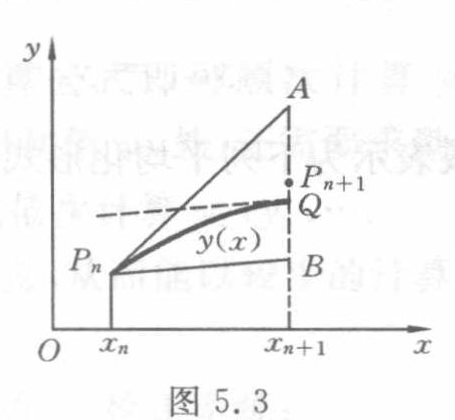
\includegraphics[width=0.85\linewidth,height=\textheight,keepaspectratio,alt={图 5.3 原图}]{../assets/ch05a/fig-5.3.png}

图 5.3（原图）：\(P_n\) 出发的两条线分别交 \(x=x_{n+1}\) 于 \(A,B\)，取平均所得点为 \(P_{n+1}\)；积分曲线标为 \(y(x)\)。原图全部标签：\(O,\allowbreak x,\allowbreak y,\allowbreak x_n,\allowbreak x_{n+1},\allowbreak P_n,\allowbreak A,\allowbreak B,\allowbreak P_{n+1},\allowbreak Q,\allowbreak y(x)\)。

\href{../../source-images/pdf-123.jpeg}{原页}

点 \(Q\) 比较远，然而从图形上可以明显地看出，\(AB\) 的中点 \(P_{n+1}\) 相当接近点 \(Q\)，可见梯形方法确实改善了精度（这里的解释不够严密，然而是令人信服的）。

梯形方法是隐式的，可用迭代法求解。同后退的 Euler 方法一样，仍用 Euler 方法提供迭代初值，则梯形法的迭代公式为

\[
\begin{cases}
y_{n+1}^{(0)}=y_n+hf(x_n,y_n),\\
y_{n+1}^{(k+1)}=y_n+\dfrac{h}{2}[f(x_n,y_n)+f(x_{n+1},y_{n+1}^{(k)})]
\end{cases}
\quad(k=0,1,2,\cdots).\tag{5.2.9}
\]

为了分析迭代过程的收敛性，将式 (5.2.8) 与式 (5.2.9) 相减，得

\[
y_{n+1}-y_{n+1}^{(k+1)}=\frac{h}{2}[f(x_{n+1},y_{n+1})-f(x_{n+1},y_{n+1}^{(k)})],
\]

于是有

\[
|y_{n+1}-y_{n+1}^{(k+1)}|\leqslant\frac{hL}{2}|y_{n+1}-y_{n+1}^{(k)}|,
\]

其中 \(L\) 为 \(f(x,y)\) 关于 \(y\) 的 Lipschitz 常数。如果选取 \(h\) 充分小，使得 \(\dfrac{hL}{2}<1\)，则当 \(k\to\infty\) 时有 \(y_{n+1}^{(k)}\to y_{n+1}\)，这说明迭代过程 (5.2.9) 是收敛的（关于迭代法的收敛性，可参见 6.2 节）。

\subsubsection{5.2.4 改进的 Euler 格式}\label{ux6539ux8fdbux7684-euler-ux683cux5f0f}

我们看到，梯形方法虽然提高了精度，但其算法复杂，在应用迭代公式 (5.2.9) 进行实际计算时，每迭代一次，都要重新计算函数 \(f\) 的值，而迭代又要反复进行若干次，计算量很大，而且往往难以预测。为了控制计算量，通常希望只迭代一两次就转入下一步计算，从而简化算法。

具体地说，先用 Euler 格式求得一个初步的近似值 \(\bar y_{n+1}\)，称之为\textbf{预测值}。预测值 \(\bar y_{n+1}\) 的精度可能很差，再用梯形公式 (5.2.8) 将它校正一次，即按式 (5.2.9) 迭代一次，得 \(y_{n+1}\)，这个结果称为\textbf{校正值}。而这样建立的预测-校正系统通常称为\textbf{改进的 Euler 格式}：

预测

\[
\bar y_{n+1}=y_n+hf(x_n,y_n),\tag{5.2.10}
\]

校正

\[
y_{n+1}=y_n+\frac{h}{2}[f(x_n,y_n)+f(x_{n+1},\bar y_{n+1})].\tag{5.2.11}
\]

这一计算格式亦可表示为

\[
y_{n+1}=y_n+\frac{h}{2}[f(x_n,y_n)+f(x_n+h,y_n+hf(x_n,y_n))],\tag{5.2.12}
\]

或表示为下列平均化形式：

\[
\begin{cases}
y_p=y_n+hf(x_n,y_n),\\
y_c=y_n+hf(x_{n+1},y_p),\\
y_{n+1}=\dfrac{1}{2}(y_p+y_c).
\end{cases}
\]

\href{../../source-images/pdf-124.jpeg}{原页}

\textbf{例 5.2} 用改进的 Euler 方法求解初值问题 (5.2.2)。

\textbf{解} 改进的 Euler 格式为

\[
\begin{cases}
y_p=y_n+h\left(y_n-\dfrac{2x_n}{y_n}\right),\\
y_c=y_n+h\left(y_p-\dfrac{2x_{n+1}}{y_p}\right),\\
y_{n+1}=\dfrac{1}{2}(y_p+y_c).
\end{cases}
\]

仍取 \(h=0.1\)，计算结果如表 5.2 所示。与例 5.1 Euler 方法的计算结果比较，改进的 Euler 方法明显地改善了精度。

\textbf{表 5.2}

{\def\LTcaptype{none} % do not increment counter
\begin{longtable}[]{@{}llllll@{}}
\toprule\noalign{}
\(x_n\) & \(y_n\) & \(y(x_n)\) & \(x_n\) & \(y_n\) & \(y(x_n)\) \\
\midrule\noalign{}
\endhead
\bottomrule\noalign{}
\endlastfoot
0.1 & 1.0959 & 1.0954 & 0.6 & 1.4860 & 1.4832 \\
0.2 & 1.1841 & 1.1832 & 0.7 & 1.5525 & 1.5492 \\
0.3 & 1.2662 & 1.2649 & 0.8 & 1.6153 & 1.6125 \\
0.4 & 1.3434 & 1.3416 & 0.9 & 1.6782 & 1.6733 \\
0.5 & 1.4164 & 1.4142 & 1.0 & 1.7379 & 1.7321 \\
\end{longtable}
}

\subsubsection{5.2.5 Euler 两步格式}\label{euler-ux4e24ux6b65ux683cux5f0f}

再考察改进的 Euler 格式 (5.2.10)、(5.2.11)，可以看到，其预测公式（Euler 格式）的精度差，与校正公式（梯形格式）不匹配。现在构造能与梯形方法在精度上相匹配的显式方法，为此改用中心差商 \(\dfrac{y(x_{n+1})-y(x_{n-1})}{2h}\) 替代方程 (5.2.4) 左端的导数项 \(y'(x_n)\)，这时离散化得到所谓 \textbf{Euler 两步格式}

\[
y_{n+1}=y_{n-1}+2hf(x_n,y_n).\tag{5.2.13}
\]

前面介绍过的数值方法，无论是 Euler 方法、后退的 Euler 方法，还是改进的 Euler 方法，它们都是\textbf{单步法}，其特点是在计算 \(y_{n+1}\) 时只用到前面一步的信息 \(y_n\)；然而，Euler 两步格式除了含 \(y_n\) 外，还显含更前面一步的信息 \(y_{n+1}\)------即调用了前面两步的信息，\textbf{Euler 两步法}因此而得名。

单步法的优点是``自开始''，只要给出初值 \(y_0\)，依计算公式即可顺次计算 \(y_1,y_2,\cdots\)。然而两步法不是自开始的，在实际计算时，除了给出初值 \(y_0\) 外，还需要求助于其他单步法再提供一个\textbf{开始值} \(y_1\)，然后才能启动计算公式依次计算 \(y_2,y_3,\cdots\)。

两步法的优点是，由于它调用了两个节点上的已知信息，从而能以较少的计算量获得较高的精度。

现在用 Euler 两步格式与梯形格式相匹配，得到如下预测-校正系统：

\begin{quote}
\textbf{校注（agent 补充，原书疑误）}：表 5.2 在 \(x_n=0.8\) 的 \(y_n\) 原印为 \(1.6153\)，已按原图保留。按例 5.2 所列递推式从 \(y_0=1\)、\(h=0.1\) 计算，得 \(y_7=1.5525140913\cdots\)、\(y_8=1.6164747827\cdots\)，保留四位小数应为 \(1.6165\)。这是原书数值疑误，非 OCR 修正；其余各行按同一计算与表中四位小数相符。

\textbf{校注（agent 补充，原书下标错误）}：本页``两步格式''说明中的``更前面一步的信息 \(y_{n+1}\)''原图确实印为 \(n+1\)；按紧邻的式 (5.2.13)，此处应指 \(y_{n-1}\)。正文保留原印下标。
\end{quote}

\href{../../source-images/pdf-125.jpeg}{原页}

预测

\[
\bar y_{n+1}=y_{n-1}+2hf(x_n,y_n),\tag{5.2.14}
\]

校正

\[
y_{n+1}=y_n+\frac{h}{2}[f(x_n,y_n)+f(x_{n+1},\bar y_{n+1})].\tag{5.2.15}
\]

与改进的 Euler 格式 (5.2.10)、(5.2.11) 比较，系统 (5.2.14)、(5.2.15) 的一个突出的特点是，它的预测公式与校正公式具有同等精度。下面将会看到，据此能比较方便地估计出截断误差，并且基于这种估计，可以提供一种提高精度的简易方法。

截断误差的分析仍用 Taylor 方法。假设预测公式 (5.2.14) 中的 \(y_n\) 和 \(y_{n-1}\) 都是准确的，即 \(y_n=y(x_n)\)，\(y_{n-1}=y(x_{n-1})\)，则容易验证其局部截断误差

\[
y(x_{n+1})-\bar y_{n+1}\approx\frac{h^3}{3}y'''(x_n).\tag{5.2.16}
\]

此外，在分析校正公式 (5.2.15) 的误差时，假定其中的预测值 \(\bar y_{n+1}\) 是准确的，即 \(\bar y_{n+1}=y(x_{n+1})\)，这时有

\[
y(x_{n+1})-y_{n+1}\approx-\frac{h^3}{12}y'''(x_n).\tag{5.2.17}
\]

比较式 (5.2.16) 和式 (5.2.17) 可发现，校正值的误差 \(y(x_{n+1})-y_{n+1}\) 大约只有预测值的误差 \(y(x_{n+1})-\bar y_{n+1}\) 的 \(1/4\)（注意符号相反），即有

\[
\frac{y(x_{n+1})-y_{n+1}}{y(x_{n+1})-\bar y_{n+1}}\approx-\frac{1}{4}.
\]

由此可导出下列事后估计式：

\[
\begin{cases}
y(x_{n+1})-\bar y_{n+1}\approx-\dfrac{4}{5}(\bar y_{n+1}-y_{n+1}),\\
y(x_{n+1})-y_{n+1}\approx\dfrac{1}{5}(\bar y_{n+1}-y_{n+1}).
\end{cases}\tag{5.2.18}
\]

可以期望，利用这样估计出的误差作为计算结果的一种补偿，有可能使精度得到改善。

设以 \(p_n\) 和 \(c_n\) 分别表示第 \(n\) 步的预测值和校正值，按估计式 (5.2.18)，\(p_{n+1}-\dfrac{4}{5}(p_{n+1}-c_{n+1})\) 和 \(c_{n+1}+\dfrac{1}{5}(p_{n+1}-c_{n+1})\) 分别可以取作 \(p_{n+1}\) 和 \(c_{n+1}\) 的改进值。在校正值 \(c_{n+1}\) 尚未求出之前，可用上一步的偏差值 \(p_n-c_n\) 替代 \(p_{n+1}-c_{n+1}\) 来改进预测值 \(p_{n+1}\)，这样设计的计算方案共有六个环节：

预测

\[
p_{n+1}=y_{n-1}+2hy'_n,
\]

改进

\[
m_{n+1}=p_{n+1}-\frac{4}{5}(p_n-c_n),
\]

计算

\[
m'_{n+1}=f(x_{n+1},m_{n+1}),
\]

校正

\[
c_{n+1}=y_n+\frac{h}{2}(m'_{n+1}+y'_n),
\]

改进

\[
y_{n+1}=c_{n+1}+\frac{1}{5}(p_{n+1}-c_{n+1}),
\]

\href{../../source-images/pdf-126.jpeg}{原页}

计算

\[
y'_{n+1}=f(x_{n+1},y_{n+1}).
\]

运用上述方案计算 \(y_{n+1}\) 时，要用到先一步的信息 \(y_n,y'_n,p_n-c_n\) 和更前一步的信息 \(y_{n-1}\)，因此在启动计算之前必须给出开始值 \(y_1\) 和 \(p_1-c_1\)，\(y_1\) 可用其他单步法（例如改进的 Euler 方法）来计算，\(p_1-c_1\) 则一般令它等于零。（计算的实践表明，这种简单的处理方法通常可以获得令人满意的效果。）

\subsection{5.3 Runge-Kutta 方法}\label{runge-kutta-ux65b9ux6cd5}

本节介绍一类高精度的单步法------Runge-Kutta 方法。这类方法与下述 Taylor 级数法有着紧密的联系。

\subsubsection{5.3.1 Taylor 级数法}\label{taylor-ux7ea7ux6570ux6cd5}

设初值问题 (5.1.1)、(5.1.2) 有解 \(y=y(x)\)，用 Taylor 展开，有

\[
y(x_{n+1})=y(x_n)+hy'(x_n)+\frac{h^2}{2!}y''(x_n)+\frac{h^3}{3!}y'''(x_n)+\cdots,\tag{5.3.1}
\]

其中 \(y(x)\) 的各阶导数依据所给方程 (5.1.1) 可以用函数 \(f\) 来表达。下面引进函数序列 \(f^{(j)}(x,y)\) 来描述求导过程，即

\[
y'=f\equiv f^{(0)},\qquad
y''=\frac{\partial f^{(0)}}{\partial x}+f\frac{\partial f^{(0)}}{\partial y}\equiv f^{(1)},\qquad
y'''=\frac{\partial f^{(1)}}{\partial x}+f\frac{\partial f^{(1)}}{\partial y}\equiv f^{(2)},\qquad\cdots.
\]

一般地

\[
y^{(j)}=\frac{\partial f^{(j-2)}}{\partial x}+f\frac{\partial f^{(j-2)}}{\partial y}\equiv f^{(j-1)},\qquad j=2,3,\cdots,
\]

而具体写出则有

\[
\begin{cases}
y'=f,\\
y''=\dfrac{\partial f}{\partial x}+f\dfrac{\partial f}{\partial y},\\
y'''=\dfrac{\partial^2f}{\partial x^2}+2f\dfrac{\partial^2f}{\partial x\partial y}
+f^2\dfrac{\partial^2f}{\partial y^2}
+\dfrac{\partial f}{\partial y}\left(\dfrac{\partial f}{\partial x}+f\dfrac{\partial f}{\partial y}\right),\\
\qquad\vdots
\end{cases}\tag{5.3.2}
\]

在展开式 (5.3.1) 的右端截取若干项，并且在 \((x_n,y_n)\) 按式 (5.3.2) 计算系数 \(y^{(j)}(x_n)\) 的近似值 \(y_n^{(j)}\)，结果导出下列 \textbf{Taylor 格式}

\[
y_{n+1}=y_n+hy'_n+\frac{h^2}{2!}y''_n+\cdots+\frac{h^p}{p!}y_n^{(p)},\tag{5.3.3}
\]

其中一阶 Taylor 格式 \((p=1)\)

\[
y_{n+1}=y_n+hy'_n
\]

就是 Euler 格式，而提高 Taylor 格式的阶 \(p\) 即可提高计算结果的精度。显然，\(p\) 阶

\href{../../source-images/pdf-127.jpeg}{原页}

Taylor 格式 (5.3.3) 的局部截断误差为

\[
y(x_{n+1})-y_{n+1}=\frac{h^{p+1}}{(p+1)!}y^{(p+1)}(\xi),\qquad x_n<\xi<x_{n+1},
\]

因此，它按下述定义具有 \(p\) 阶精度。

\textbf{定义 5.1} 如果一种方法的局部截断误差为 \(O(h^{p+1})\)，则称该方法具有 \(p\) 阶精度。

\textbf{例 5.3} 用 Taylor 级数法求解例 5.1 的初值问题 (5.2.2)。

\textbf{解} 直接求导知

\[
\begin{aligned}
y'&=y-\frac{2x}{y},\\
y''&=y'-\frac{2}{y^2}(y-xy'),\\
y'''&=y''+\frac{2}{y^2}(xy''+2y')-\frac{4x(y')^2}{y^3},\\
y^{(4)}&=y'''+\frac{2}{y^2}(xy'''+3y'')-\frac{12y'}{y^3}(xy''+y')+\frac{12x(y')^3}{y^4}.
\end{aligned}
\]

据此用四阶 Taylor 格式即可获得令人满意的结果（仍取步长 \(=0.1\) 计算，结果如表 5.3 所示）。

\textbf{表 5.3}

{\def\LTcaptype{none} % do not increment counter
\begin{longtable}[]{@{}lll@{}}
\toprule\noalign{}
\(x_n\) & \(y_n\) & \(y(x_n)\) \\
\midrule\noalign{}
\endhead
\bottomrule\noalign{}
\endlastfoot
0.1 & 1.0954 & 1.0954 \\
0.2 & 1.1832 & 1.1832 \\
0.3 & 1.2649 & 1.2649 \\
\end{longtable}
}

应当指出，Taylor 格式 (5.3.3) 从形式上看似简单，但具体构造这种格式往往是相当困难的，因为它需要按式 (5.3.2) 提供导数值 \(y_n^{(j)}\)。当阶数提高时，求导过程式 (5.3.2) 可能很复杂，因此 Taylor 级数法通常不直接使用，但可以用它来启发思路。

\subsubsection{5.3.2 Runge-Kutta 方法的基本思想}\label{runge-kutta-ux65b9ux6cd5ux7684ux57faux672cux601dux60f3}

Runge-Kutta 方法实质上是间接地使用 Taylor 级数法的一种方法。

考察差商 \(\dfrac{y(x_{n+1})-y(x_n)}{h}\)，根据微分中值定理，存在 \(0<\theta<1\)，使得

\[
\frac{y(x_{n+1})-y(x_n)}{h}=y'(x_n+\theta h),
\]

于是，利用所给方程 \(y'=f(x,y)\) 得到

\[
y(x_{n+1})=y(x_n)+hf(x_n+\theta h,y(x_n+\theta h)).\tag{5.3.4}
\]

设 \(K^*=f(x_n+\theta h,y(x_n+\theta h))\)，称 \(K^*\) 为区间 \([x_n,x_{n+1}]\) 上的\textbf{平均斜率}。由此可见，只要对平均斜率提供一种算法，那么由式 (5.3.4) 便相应地导出一种计算格式。

Euler 格式 (5.2.1) 简单地取点 \(x_n\) 的斜率值 \(K_1=f(x_n,y_n)\) 作为平均斜率 \(K^*\)，

\href{../../source-images/pdf-128.jpeg}{原页}

精度自然很低。

再考察改进的 Euler 格式 (5.2.10)、(5.2.11)，它可改写成下列平均化的形式：

\[
\begin{cases}
y_{n+1}=y_n+\dfrac{h}{2}(K_1+K_2),\\
K_1=f(x_n,y_n),\\
K_2=f(x_{n+1},y_n+hK_1).
\end{cases}
\]

可见，改进的 Euler 格式可以这样理解：它用 \(x_n\) 与 \(x_{n+1}\) 两个点的斜率值 \(K_1\) 与 \(K_2\) 取算术平均作为平均斜率 \(K^*\)，而 \(x_{n+1}\) 处的斜率值 \(K_2\) 则通过已知信息 \(y_n\) 来预测。

这个处理过程启示我们，如果设法在 \((x_n,x_{n+1})\) 内多预测几个点的斜率值，然后将它们加权平均作为平均斜率 \(K^*\)，则有可能构造出具有更高精度的计算格式。这就是 Runge-Kutta 方法的基本思想。

\subsubsection{5.3.3 二阶 Runge-Kutta 方法}\label{ux4e8cux9636-runge-kutta-ux65b9ux6cd5}

首先推广改进的 Euler 方法，随意考察区间 \((x_n,x_{n+1})\) 内一点

\[
x_{n+p}=x_n+ph,\qquad 0<p\leqslant1,
\]

希望用 \(x_n\) 和 \(x_{n+p}\) 两个点的斜率值 \(K_1\) 和 \(K_2\) 线性组合得到平均斜率 \(K^*\)，即令

\[
y_{n+1}=y_n+h(\lambda_1K_1+\lambda_2K_2),
\]

其中 \(\lambda_1,\lambda_2\) 为待定系数。同改进的 Euler 格式一样，这里仍取 \(K_1=f(x_n,y_n)\)，问题在于该怎样预测 \(x_{n+p}\) 处的斜率值 \(K_2\)。

仿照改进的 Euler 格式，先用 Euler 格式提供 \(y(x_{n+p})\) 的预测值，即

\[
y_{n+p}=y_n+phK_1,
\]

然后再用预测值 \(y_{n+p}\) 通过计算 \(f\) 产生斜率值

\[
K_2=f(x_{n+p},y_{n+p}).
\]

这样设计出的计算格式具有如下形式：

\[
\begin{cases}
y_{n+1}=y_n+h(\lambda_1K_1+\lambda_2K_2),\\
K_1=f(x_n,y_n),\\
K_2=f(x_{n+p},y_n+phK_1).
\end{cases}\tag{5.3.5}
\]

式 (5.3.5) 含有三个待定系数 \(\lambda_1,\lambda_2\) 和 \(p\)，希望适当选取这些系数的值，使得格式具有二阶精度。

根据式 (5.3.3)，二阶 Taylor 格式为

\[
y_{n+1}=y_n+hy'_n+\frac{h^2}{2}y''_n,
\]

或表示为

\[
y_{n+1}=y_n+hf_n+\frac{h^2}{2}(f_x+f\cdot f_y)_n,
\]

其中 \(f_n\) 和 \((f_x+f\cdot f_y)_n\) 的下标 \(n\) 均表示在 \((x_n,y_n)\) 取值。另一方面，有

\href{../../source-images/pdf-129.jpeg}{原页}

\[
K_1=f_n,\qquad K_2=f(x_{n+p},y_n+phK_1)=f_n+ph(f_x+f\cdot f_y)_n+\cdots,
\]

代入式 (5.3.5)，得

\[
y_{n+1}=y_n+(\lambda_1+\lambda_2)hf_n+\lambda_2ph^2(f_x+f\cdot f_y)_n+\cdots.
\]

由此可见，欲使格式 (5.3.5) 具有二阶精度，只要成立

\[
\begin{cases}
\lambda_1+\lambda_2=1,\\
\lambda_2p=\dfrac{1}{2}.
\end{cases}\tag{5.3.6}
\]

满足条件 (5.3.6) 的一族格式 (5.3.5) 统称为\textbf{二阶 Runge-Kutta 格式}。

除了改进的 Euler 格式外，另一种特殊的二阶 Runge-Kutta 格式是所谓\textbf{变形的 Euler 格式}，其形式如下：

\[
\begin{cases}
y_{n+1}=y_n+hK_2,\\
K_1=f(x_n,y_n),\\
K_2=f\left(x_n+\dfrac{h}{2},y_n+\dfrac{h}{2}K_1\right).
\end{cases}
\]

表面上看，变形的 Euler 格式 \(y_{n+1}=y_n+hK_2\) 仅显含一个斜率值 \(K_2\)，但 \(K_2\) 是通过 \(K_1\) 计算出来的，因此每完成一步仍然需要两次计算函数 \(f\) 的值，工作量和改进的 Euler 格式相同。

总之，二阶 Runge-Kutta 方法用多算一次函数值 \(f\) 的办法，避开了二阶 Taylor 级数法所要求的 \(f\) 导数值的计算。在这种意义上可以说，Runge-Kutta 方法实质上是 Taylor 方法的变形。

\subsubsection{5.3.4 三阶 Runge-Kutta 方法}\label{ux4e09ux9636-runge-kutta-ux65b9ux6cd5}

为了进一步提高精度，设除 \(x_n,x_{n+p}\) 外再考察一点 \(x_{n+p}=x_n+qh\)，\(p\leqslant q\leqslant1\)，并用三个点 \(x_n,x_{n+p},x_{n+q}\) 的斜率值 \(K_1,K_2,K_3\) 线性组合得到平均斜率 \(K^*\)，这时计算格式为

\[
y_{n+1}=y_n+h(\lambda_1K_1+\lambda_2K_2+\lambda_3K_3).
\]

其中 \(K_1,K_2\) 仍用格式 (5.3.5) 所取的形式。

为了预测点 \(x_{n+p}\) 处的斜率值 \(K_3\)，在区间 \((x_n,x_{n+q})\) 内有两个斜率值 \(K_1\) 和 \(K_2\) 可以利用。用 \(K_1\) 和 \(K_2\) 线性组合给出区间 \([x_n,x_{n+q}]\) 上的平均斜率，从而得到 \(y(x_{n+q})\) 的预测值 \(y_{n+q}=y_n+qh(rK_1+sK_2)\)，于是，再通过计算函数值 \(f\) 得到

\[
K_3=f(x_{n+q},y_{n+q})=f(x_n+qh,y_n+qh(rK_1+sK_2)).
\]

这样设计出的计算格式具有如下形式：

\[
\begin{cases}
y_{n+1}=y_n+h(\lambda_1K_1+\lambda_2K_2+\lambda_3K_3),\\
K_1=f(x_n,y_n),\\
K_2=f(x_n+ph,y_n+phK_1),\\
K_3=f(x_n+qh,y_n+qh(rK_1+sK_2)).
\end{cases}\tag{5.3.7}
\]

\begin{quote}
\textbf{校注（agent 补充，原书下标错误）}：5.3.4 首段``再考察一点 \(x_{n+p}=x_n+qh\)''及后段``为了预测点 \(x_{n+p}\) 处的斜率值 \(K_3\)''，原图两处均印为 \(n+p\)，已保留。按同页对 \(K_3=f(x_{n+q},y_{n+q})\) 的定义及式 (5.3.7)，这两处所指节点均应为 \(x_{n+q}\)。已放大原印字确认，非 OCR 误识。
\end{quote}

\href{../../source-images/pdf-130.jpeg}{原页}

希望适当选择系数 \(\lambda_1,\lambda_2,\lambda_3\) 和 \(p,q,r,s\)，能使上述格式具有三阶精度。

为便于进行数学演算，引进算子

\[
\mathrm D=\frac{\partial}{\partial x}+f\frac{\partial}{\partial y},\qquad
\mathrm D^2=\frac{\partial^2}{\partial x^2}+2f\frac{\partial^2}{\partial x\partial y}+f^2\frac{\partial^2}{\partial y^2},
\]

则根据式 (5.3.2)，有

\[
y'=f,\qquad y''=\mathrm Df,\qquad y'''=\mathrm D^2f+\frac{\partial f}{\partial y}\mathrm Df,
\]

于是三阶 Taylor 格式

\[
y_{n+1}=y_n+hy'_n+\frac{h^2}{2}y''_n+\frac{h^3}{6}y'''_n
\]

可表示为

\[
y_{n+1}=y_n+hf_n+\frac{h^2}{2}\mathrm Df_n+\frac{h^3}{6}(\mathrm D^2f+f_y\mathrm Df)_n,\tag{5.3.8}
\]

其中 \(f_n,\mathrm Df_n\) 等的下标 \(n\) 均表示在 \((x_n,y_n)\) 取值。

另一方面，再将式 (5.3.7) Taylor 展开，其中

\[
K_1=f_n,
\]

\[
K_2=f(x_n+ph,y_n+phK_1)=f_n+ph\mathrm Df_n+\frac{(ph)^2}{2}\mathrm D^2f_n+\cdots,
\]

\[
K_3=f(x_n+qh,y_n+qh(rK_1+sK_2))=f_n+qh\overline{\mathrm D}f_n+\frac{(qh)^2}{2}\overline{\mathrm D}^{2}f_n+\cdots.
\]

这里，算子 \(\overline{\mathrm D}=\dfrac{\partial}{\partial x}+(rK_1+sK_2)\dfrac{\partial}{\partial y}\)。

若取

\[
r+s=1,\tag{5.3.9}
\]

则易知

\[
\overline{\mathrm D}=\mathrm D+hps\mathrm Df_n\frac{\partial}{\partial y}+\cdots,\tag{5.3.10}
\]

\[
\overline{\mathrm D}^{2}=\mathrm D^2+\cdots,
\]

因此

\[
K_3=f_n+qh\mathrm Df_n+\frac{h^2}{2}(q^2\mathrm D^2f+2pqs\mathrm Df\cdot f_y)_n+\cdots.
\]

将以上 \(K_1,K_2,K_3\) 的展开式一起代入式 (5.3.7)，再令

\[
\lambda_1+\lambda_2+\lambda_3=1,\tag{5.3.11}
\]

则有

\[
\begin{aligned}
y_{n+1}={}&y_n+hf_n+h^2(\lambda_2p+\lambda_3q)\mathrm Df_n\\
&+h^3\left(\frac12\lambda_2p^2\mathrm D^2f+\frac12\lambda_3q^2\mathrm D^2f+\lambda_3pqsf_y\mathrm Df\right)_n+\cdots,
\end{aligned}
\]

于是为了保证它能与三阶 Taylor 格式 (5.3.8) 具有同等精度，只要满足下列方程组：

\[
\begin{cases}
\lambda_2p+\lambda_3q=\dfrac12,\\
\lambda_2p^2+\lambda_3q^2=\dfrac13,\\
\lambda_3pqs=\dfrac16.
\end{cases}\tag{5.3.12}
\]

\href{../../source-images/pdf-131.jpeg}{原页}

满足条件 (5.3.9)、(5.3.11)、(5.3.12) 的一族格式 (5.3.7) 统称\textbf{三阶 Runge-Kutta 格式}。下列 Kutta 格式是其中的一个特例：

\[
\begin{cases}
y_{n+1}=y_n+\dfrac{h}{6}(K_1+4K_2+K_3),\\
K_1=f(x_n,y_n),\\
K_2=f\left(x_n+\dfrac{h}{2},y_n+\dfrac{h}{2}K_1\right),\\
K_3=f(x_n+h,y_n-hK_1+2hK_2).
\end{cases}
\]

\subsubsection{5.3.5 四阶 Runge-Kutta 方法}\label{ux56dbux9636-runge-kutta-ux65b9ux6cd5}

继续上述过程，经过较复杂的数学演算，可以导出各种四阶 Runge-Kutta 格式，下列\textbf{经典格式}是其中常用的一个：

\[
\begin{cases}
y_{n+1}=y_n+\dfrac{h}{6}(K_1+2K_2+2K_3+K_4),\\
K_1=f(x_n,y_n),\\
K_2=f\left(x_n+\dfrac{h}{2},y_n+\dfrac{h}{2}K_1\right),\\
K_3=f\left(x_n+\dfrac{h}{2},y_n+\dfrac{h}{2}K_2\right),\\
K_4=f(x_n+h,y_n+hK_3).
\end{cases}\tag{5.3.13}
\]

四阶 Runge-Kutta 方法的每一步需要四次计算函数值 \(f\)，可以证明其截断误差为 \(O(h^5)\)。其证明极其烦琐，这里从略。

\textbf{例 5.4} 设取步长 \(h=0.2\)，从 \(x=0\) 直到 \(x=1\) 用四阶 Runge-Kutta 方法求解初值问题 (5.2.2)。

\textbf{解} 这里，经典的四阶 Runge-Kutta 格式 (5.3.13) 具有如下形式：

\[
\begin{cases}
y_{n+1}=y_n+\dfrac{h}{6}(K_1+2K_2+2K_3+K_4),\\
K_1=y_n-\dfrac{2x_n}{y_n},\\
K_2=y_n+\dfrac{h}{2}K_1-\dfrac{2x_n+h}{y_n+\dfrac{h}{2}K_1},\\
K_3=y_n+\dfrac{h}{2}K_2-\dfrac{2x_n+h}{y_n+\dfrac{h}{2}K_2},\\
K_4=y_n+hK_3-\dfrac{2(x_n+h)}{y_n+hK_3}.
\end{cases}
\]

表 5.4 列出计算结果 \(y_n\)，其中 \(y(x_n)\) 仍表示准确解。

\href{../../source-images/pdf-132.jpeg}{原页}

比较例 5.4 和例 5.2 的计算结果，显然以四阶 Runge-Kutta 方法的精度为高。注意，虽然四阶 Runge-Kutta 方法的计算量（每一步要四次计算函数 \(f\)）比改进的 Euler 方法（它是一种二阶 Runge-Kutta 方法，每一步只要两次计算函数 \(f\)）大一倍，但由于这里放大了步长 \((h=0.2)\)，造出表 5.4 和表 5.2 所耗费的计算量几乎相同。这个例子又一次显示了选择算法的重要意义。

\textbf{表 5.4}

{\def\LTcaptype{none} % do not increment counter
\begin{longtable}[]{@{}lll@{}}
\toprule\noalign{}
\(x_n\) & \(y_n\) & \(y(x_n)\) \\
\midrule\noalign{}
\endhead
\bottomrule\noalign{}
\endlastfoot
0.2 & 1.1832 & 1.1832 \\
0.4 & 1.3417 & 1.3416 \\
0.6 & 1.4833 & 1.4832 \\
0.8 & 1.6125 & 1.6125 \\
1.0 & 1.7321 & 1.7321 \\
\end{longtable}
}

然而值得指出的是，Runge-Kutta 方法的推导基于 Taylor 展开方法，因而它要求所求的解具有较好的光滑性质。反之，如果解的光滑性差，那么，使用四阶 Runge-Kutta 方法可能反而不如使用改进的 Euler 方法求得的数值解的精度高。实际计算时，应当针对问题的具体特点选择合适的算法。

\subsubsection{5.3.6 变步长的 Runge-Kutta 方法}\label{ux53d8ux6b65ux957fux7684-runge-kutta-ux65b9ux6cd5}

单从每一步看，步长越小，截断误差就越小；但随着步长的缩小，在一定求解范围内所要完成的步数就增加了。步数的增加不但引起计算量的增大，而且可能导致舍入误差的严重积累。因此同积分的数值计算一样，微分方程的数值解法也有个选择步长的问题。

在选择步长时，需要考虑两个问题：

（1）怎样衡量和检验计算结果的精度？

（2）如何依据所获得的精度处理步长？

考察经典的四阶 Runge-Kutta 格式 (5.3.13)。从节点 \(x_n\) 出发，先以 \(h\) 为步长求出一个近似值，作为 \(y_{n+1}^{(h)}\)，由于格式的局部截断误差为 \(O(h^5)\)，故有

\[
y(x_{n+1})-y_{n+1}^{(h)}\approx Ch^5;\tag{5.3.14}
\]

然后将步长折半，即取 \(\dfrac{h}{2}\) 为步长从 \(x_n\) 跨两步到 \(x_{n+1}\)，再求得一个近似值 \(y_{n+1}^{(h/2)}\)，每跨一步的截断误差是 \(C\left(\dfrac{h}{2}\right)^5\)，因此有

\[
y(x_{n+1})-y_{n+1}^{(h/2)}=2C\left(\frac{h}{2}\right)^5;\tag{5.3.15}
\]

比较式 (5.3.14) 和式 (5.3.15) 可以看到，步长折半后，误差大约减小到 \(\dfrac{1}{16}\)，即有

\[
\frac{y(x_{n+1})-y_{n+1}^{(h/2)}}{y(x_{n+1})-y_{n+1}^{(h)}}\approx\frac{1}{16}.
\]

由此易得下列事后估计式

\[
y(x_{n+1})-y_{n+1}^{(h/2)}\approx\frac{1}{15}(y_{n+1}^{(h/2)}-y_{n+1}^{(h)}).
\]

\href{../../source-images/pdf-133.jpeg}{原页}

这样，可以通过检查步长折半前后两次计算结果的偏差

\[
\Delta=|y_{n+1}^{(h/2)}-y_{n+1}^{(h)}|
\]

来判定所选的步长是否合适。具体地说，将分以下两种情况处理：

（1）对于给定的精度 \(\varepsilon\)，如果 \(\Delta>\varepsilon\)，应反复将步长折半进行计算，直至 \(\Delta<\varepsilon\) 为止，这时取最终得到的 \(y_{n+1}^{(h/2)}\) 作为结果；

（2）如果 \(\Delta<\varepsilon\)，则反复将步长加倍，直至 \(\Delta>\varepsilon\) 为止，这时再将步长折半一次，就得到所要的结果。

这种通过加倍或折半处理步长的方法称为\textbf{变步长方法}。表面上看，为了选择步长，每一步的计算量增加了，但从总体考虑往往是合算的。

\subsection{5.4 单步法的收敛性和稳定性}\label{ux5355ux6b65ux6cd5ux7684ux6536ux655bux6027ux548cux7a33ux5b9aux6027}

\subsubsection{5.4.1 单步法的收敛性}\label{ux5355ux6b65ux6cd5ux7684ux6536ux655bux6027}

我们看到，数值解法的基本思想是，通过某种离散化手段，将微分方程转化为差分方程（代数方程）来求解。这种转化是否合理，还要看差分问题的解 \(y_n\) 当 \(h\to0\) 时是否会收敛到微分方程的准确解 \(y(x_n)\)。需要注意的是，如果只考虑 \(h\to0\)，那么节点 \(x_n=x_0+nh\) 对于固定的 \(n\) 将趋于 \(x_0\)，这时讨论收敛性是没有意义的。

\textbf{定义 5.2} 若一种数值方法对于任意固定的 \(x_n=x_0+nh\)，当 \(h\to0\)（同时 \(n\to\infty\)）时有 \(y_n\to y(x_n)\)，则称该方法是\textbf{收敛的}。

先就简单的初值问题

\[
\begin{cases}
y'=\lambda y,\\
y(0)=y_0
\end{cases}\tag{5.4.1}
\]

考察 Euler 方法的收敛性。方程 \(y'=\lambda y\) 的 Euler 格式是

\[
y_{n+1}=(1+\lambda h)y_n,\tag{5.4.2}
\]

它显然有解

\[
y_n=y_0(1+\lambda h)^n.
\]

由于这里 \(x_0=0,x_n=nh\)，有

\[
y_n=y_0\left[(1+\lambda h)^{\frac{1}{\lambda h}}\right]^{\lambda x_n}.
\]

再注意到当 \(h\to0\) 时，有

\[
(1+\lambda h)^{\frac{1}{\lambda h}}\to e,
\]

差分方程的解 \(y_n\) 当 \(h\to0\) 时确定收敛到原微分方程的准确解

\[
y(x_n)=y_0e^{\lambda x_n}.
\]

下面进一步考察一般的单步法。

所谓单步法，就是在计算 \(y_{n+1}\) 时只用到它前一步的信息 \(y_n\)。Taylor 级数法、

\href{../../source-images/pdf-134.jpeg}{原页}

Runge-Kutta 方法等都是单步法的例子。显式单步法的共同特征是，它们都是将 \(y_n\) 加上某种形式的增量得出 \(y_{n+1}\) 的，其计算公式形如

\[
y_{n+1}=y_n+h\varphi(x_n,y_n,h),\tag{5.4.3}
\]

其中 \(\varphi(x,y,h)\) 称为\textbf{增量函数}。

不同的单步法对应于不同的增量函数。不难就已知的几种单步法写出增量函数 \(\varphi(x,y,h)\) 的具体形式，譬如，对于 Euler 格式 (5.2.1)，有 \(\varphi=f(x,y)\)，而对于改进的 Euler 格式 (5.2.12)，有

\[
\varphi=\frac12[f(x,y)+f(x+h,y+hf(x,y))].\tag{5.4.4}
\]

关于单步法有下述收敛性定理。

\textbf{定理 5.1} 假设单步法 (5.4.3) 具有 \(p\) 阶精度，且增量函数 \(\varphi(x,y,h)\) 关于 \(y\) 满足 Lipschitz 条件

\[
|\varphi(x,y,h)-\varphi(x,\bar y,h)|\leqslant L_\varphi(y-\bar y),\tag{5.4.5}
\]

又设初值 \(y_0\) 是准确的，即 \(y_0=y(x_0)\)，则其\textbf{整体截断误差}

\[
y(x_n)-y_n=O(h^p).\tag{5.4.6}
\]

\textbf{证明} 设以 \(\bar y_{n+1}\) 表示取 \(y_n=y(x_n)\) 用格式 (5.4.3) 求得的结果，即

\[
\bar y_{n+1}=y(x_n)+h\varphi(x_n,y(x_n),h),\tag{5.4.7}
\]

其局部截断误差为 \(y(x_{n+1})-\bar y_{n+1}\)，由于所给方法具有 \(p\) 阶精度，按定义 5.1，存在定数 \(C\)，使

\[
|y(x_{n+1})-\bar y_{n+1}|\leqslant Ch^{p+1}.
\]

又由式 (5.4.7) 与式 (5.4.3)，得

\[
|\bar y_{n+1}-y_{n+1}|\leqslant|y(x_n)-y_n|+h|\varphi(x_n,y(x_n),h)-\varphi(x_n,y_n,h)|.
\]

利用假设条件 (5.4.5)，有

\[
|\bar y_{n+1}-y_{n+1}|\leqslant(1+hL_\varphi)|y(x_n)-y_n|,
\]

从而有

\[
\begin{aligned}
|y(x_{n+1})-y_{n+1}|&\leqslant|\bar y_{n+1}-y_{n+1}|+|y(x_{n+1})-\bar y_{n+1}|\\
&\leqslant(1+hL_\varphi)|y(x_n)-y_n|+Ch^{p+1},
\end{aligned}
\]

即对于整体截断误差 \(e_n=y(x_n)-y_n\) 成立下列递推关系式：

\[
|e_{n+1}|\leqslant(1+hL_\varphi)|e_n|+Ch^{p+1}.\tag{5.4.8}
\]

据此不等式反复递推，可得

\[
|e_n|\leqslant(1+hL_\varphi)^n|e_0|+\frac{Ch^q}{L_\varphi}[(1+hL_\varphi)^n-1].\tag{5.4.9}
\]

再注意到当 \(x_n-x_0=nh\leqslant T\) 时\footnote{对于任意实数 \(x\)，有 \(1+x\leqslant e^x\)，而当 \(x\geqslant-1\) 时，成立 \(0\leqslant(1+x)^n\leqslant e^{nx}\)。}

\begin{quote}
\textbf{校注（agent 补充，原书公式错误）}：式 (5.4.5) 原图右端为 \(L_\varphi(y-\bar y)\)，没有绝对值符号，已原样保留。标准 Lipschitz 条件及随后对非负误差的估计需要右端为 \(L_\varphi|y-\bar y|\)；当 \(y<\bar y\) 且 \(L_\varphi>0\) 时，原印右端为负，不能作为绝对差的上界。

\textbf{校注（agent 补充，原书指数错误）}：式 (5.4.9) 原印为 \(Ch^q/L_\varphi\)，已放大确认 \(q\) 并保留。按式 (5.4.8) 的等比求和，\(Ch^{p+1}\sum_{j=0}^{n-1}(1+hL_\varphi)^j=\dfrac{Ch^p}{L_\varphi}[(1+hL_\varphi)^n-1]\)，故此处指数应为 \(p\)；后页式 (5.4.10) 也用 \(p\)。
\end{quote}

\href{../../source-images/pdf-135.jpeg}{原页}

\[
(1+hL_\varphi)^n\leqslant(e^{nL_\varphi})^n\leqslant e^{hL_\varphi},
\]

最终得估计式

\[
|e_n|\leqslant|e_0|e^{TL_\varphi}+\frac{Ch^p}{L_\varphi}(e^{TL_\varphi}-1).\tag{5.4.10}
\]

由此可以断定，如果初值是准确的，即 \(e_0=0\)，则式 (5.4.6) 成立。证毕。

依据这一定理，判断单步法 (5.4.3) 的收敛性，归结为验证增量函数 \(\varphi\) 能否满足 Lipschitz 条件 (5.4.5)。

对 Euler 方法，由于其增量函数 \(\varphi\) 就是 \(f\)，故当 \(f\) 满足 Lipschitz 条件时它是收敛的。

再考察改进的 Euler 方法，其增量函数已由式 (5.4.4) 给出，这时有

\[
\begin{aligned}
&|\varphi(x,y,h)-\varphi(x,\bar y,h)|\\
&\leqslant\frac12\bigl[|f(x,y)-f(x,\bar y)|+|f(x+h,y+hf(x,y))\\
&\qquad-f(x+h,\bar y+hf(x,\bar y))|\bigr].
\end{aligned}
\]

假定 \(f\) 关于 \(y\) 满足 Lipschitz 条件，记 Lipschitz 常数为 \(L\)，则由上式推得

\[
|\varphi(x,y,h)-\varphi(x,\bar y,h)|\leqslant L\left(1+\frac{h}{2}L\right)|y-\bar y|.
\]

设限定 \(h\leqslant h_0\)（\(h_0\) 为定数），上式表明 \(\varphi\) 关于 \(y\) 的 Lipschitz 常数

\[
L_\varphi=L\left(1+\frac{h_0}{2}L\right),
\]

因此，改进的 Euler 方法也是收敛的。

类似地，不难验证其他 Runge-Kutta 方法的收敛性。

\subsubsection{5.4.2 单步法的稳定性}\label{ux5355ux6b65ux6cd5ux7684ux7a33ux5b9aux6027}

前面关于收敛性的讨论有个前提，必须假定数值方法本身的计算是准确的。实际情形并不是这样，差分方程的求解还会有计算误差，譬如由于数字舍入而引起的小扰动。这类小扰动在传播过程中会不会恶性增长，以致``淹没''了差分方程的``真解''呢？这就是差分方法的稳定性问题。在实际计算时，希望某一步产生的扰动值在后面的计算中能够被控制，甚至是逐步衰减的。

\textbf{定义 5.3} 若一种数值方法在节点值 \(y_n\) 上产生大小为 \(\delta\) 的扰动，在以后各节点值 \(y_m\)（\(m>n\)）上产生的偏差均不超过 \(\delta\)，则称该方法是\textbf{稳定的}。

稳定性问题比较复杂，为简化讨论，仅考察下列\textbf{模型方程} \(y'=\lambda y\)。为保证微分方程本身的稳定性，假定 \(\lambda<0\)。

先研究 Euler 方法的稳定性。模型方程 \(y'=\lambda y\) 的 Euler 格式为

\[
y_{n+1}=(1+h\lambda)y_n.\tag{5.4.11}
\]

设在节点值 \(y_n\) 上有一扰动值 \(\varepsilon_n\)，它的传播使节点值 \(y_{n+1}\) 产生大小为 \(\varepsilon_{n+1}\) 的扰动值，

\begin{quote}
\textbf{校注（agent 补充，原书指数错误）}：页首原印为 \((1+hL_\varphi)^n\leqslant(e^{nL_\varphi})^n\leqslant e^{hL_\varphi}\)，放大确认后按原式保留。由前页 \(nh\leqslant T\) 及 \(1+u\leqslant e^u\)，所需估计应为 \((1+hL_\varphi)^n\leqslant(e^{hL_\varphi})^n=e^{nhL_\varphi}\leqslant e^{TL_\varphi}\)，与本页式 (5.4.10) 一致。
\end{quote}

\href{../../source-images/pdf-136.jpeg}{原页}

假设用 \(y_n^*=y_n+\varepsilon_n\) 按 Euler 格式得出 \(y_{n+1}^*=y_{n+1}+\varepsilon_{n+1}\) 的计算过程不再有新的误差，则扰动值满足

\[
\varepsilon_{n+1}=(1+h\lambda)\varepsilon_n.
\]

可见扰动值满足原来的差分方程 (5.4.11)。这样，如果差分方程的解是不增长的，即有

\[
|y_{n+1}|\leqslant|y_n|,
\]

则它就是稳定的。这一论断对于下面将要研究的其他方法同样适用。

显然，为要保证差分方程 (5.4.11) 的解是不增长的，只要选取 \(h\) 充分小，使

\[
|1+h\lambda|\leqslant1.\tag{5.4.12}
\]

这说明 Euler 方法是\textbf{条件稳定的}，其稳定性条件为 \(h\leqslant-2/\lambda\)。记 \(\tau=-1/\lambda\)，则稳定性条件 (5.4.12) 可表示为

\[
h\leqslant2\tau.\tag{5.4.13}
\]

若自变量 \(x\) 表示时间，则 \(\tau\) 是一个具有时间量纲的量，工程上习惯地称它为\textbf{时间常数}。时间常数 \(\tau\) 可用来刻画原方程的解 \(y(x)\) 的衰减速度。事实上，在时间 \(\tau\) 内，解 \(y=y(0)e^{\lambda x}\) 衰减到它的 \(e^{-1}\) 倍。因此，\(\tau\) 越小，解 \(y(x)\) 衰减得越快。

Euler 方法的稳定性条件 \(h\leqslant2\tau\) 表明，时间常数 \(\tau\) 越小，稳定性对步长 \(h\) 的限制越苛刻。

再考察后退的 Euler 方法。对于模型方程 \(y'=\lambda y\)，其后退的 Euler 格式为

\[
y_{n+1}=y_n+h\lambda y_{n+1},
\]

解出 \(y_{n+1}\)，有 \(y_{n+1}=\dfrac{1}{1-h\lambda}y_n\)。由于 \(\lambda<0\)，这时恒成立

\[
\left|\frac{1}{1-h\lambda}\right|\leqslant1,
\]

从而有 \(|y_{n+1}|\leqslant|y_n|\)，因而后退的 Euler 方法\textbf{恒稳定}（或称\textbf{无条件稳定}）。

\textbf{例 5.5} 考察初值问题

\[
\begin{cases}
y'=-100y,\\
y(0)=1,
\end{cases}
\]

其准确解 \(y=e^{-100x}\) 是一个按指数曲线衰减得很快的函数，如图 5.4 所示。

对于所给方程 \(y'=-100y\)，其时间常数 \(\tau=0.01\)，因此，按式 (5.4.13)，为保证 Euler 方法稳定，步长 \(h\) 应使 \(\tau\) 不超过 \(2\tau=0.02\)。若取步长 \(h=0.025\)，则 Euler 格式的具体形式为

\[
y_{n+1}=-1.5y_n,
\]

计算结果列于表 5.5 的第二列。可以看到，Euler 方法的解 \(y_n\)（图 5.4 中用符号``■''标出）

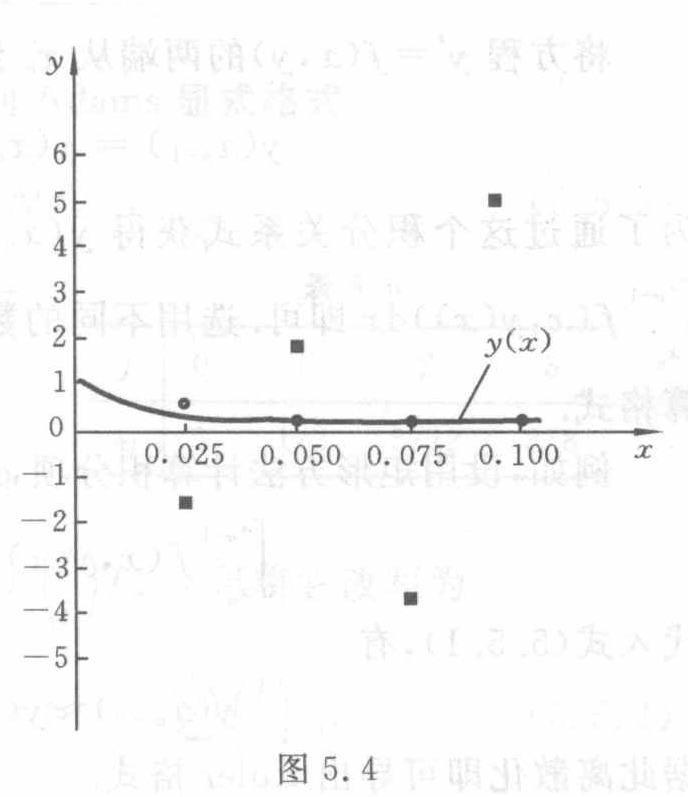
\includegraphics[width=0.85\linewidth,height=\textheight,keepaspectratio,alt={图 5.4 原图}]{../assets/ch05a/fig-5.4.png}

图 5.4（原图）：坐标系中画出衰减曲线 \(y(x)\)、正负交替且幅度增大的方形离散点，以及靠近横轴的圆形离散点。原图全部文字与刻度标签：\(x,y,y(x)\)；横轴 \(0.025,0.050,0.075,0.100\)；纵轴 \(-5,\allowbreak -4,\allowbreak -3,\allowbreak -2,\allowbreak -1,\allowbreak 0,\allowbreak 1,\allowbreak 2,\allowbreak 3,\allowbreak 4,\allowbreak 5,\allowbreak 6\)。点的说明随例 5.5 跨页续述。

\begin{quote}
\textbf{校注（agent 补充，原书文字/符号错误）}：例 5.5 原印``步长 \(h\) 应使 \(\tau\) 不超过 \(2\tau=0.02\)''，已经放大确认并保留。式 (5.4.13) 约束的是步长 \(h\)，应为``步长 \(h\) 应不超过 \(2\tau=0.02\)''；原句中的``使 \(\tau\)''使被约束量错置。
\end{quote}

\href{../../source-images/pdf-137.jpeg}{原页}

（接上页）在准确值 \(y(x_n)\) 的上下波动，计算过程明显地不稳定。

\textbf{表 5.5}

{\def\LTcaptype{none} % do not increment counter
\begin{longtable}[]{@{}lrr@{}}
\toprule\noalign{}
节点 & Euler 方法 & 后退的 Euler 方法 \\
\midrule\noalign{}
\endhead
\bottomrule\noalign{}
\endlastfoot
0.025 & −1.5 & 0.2857 \\
0.050 & 2.25 & 0.0816 \\
0.075 & −3.375 & 0.0233 \\
0.100 & 5.0625 & 0.0067 \\
\end{longtable}
}

再考察后退的 Euler 方法，取 \(h=0.025\) 时计算格式为

\[
y_{n+1}=\frac{1}{3.5}y_n.
\]

计算结果列于表 5.5 的第三列（图 5.4 中用符号``\(\bullet\)''标出），这时计算过程是稳定的。

\subsection{5.5 线性多步法}\label{ux7ebfux6027ux591aux6b65ux6cd5}

在逐步推进的求解过程中，计算 \(y_{n+1}\) 之前事实上已经求出了一系列的近似值 \(y_n,y_{n-1},y_{n-2},\cdots\)，如果充分利用前面多步的信息来预测 \(y_{n+1}\)，则可以期望会获得较高的精度。这就是构造所谓线性多步法的基本思想。

构造多步法有多种途径，下面介绍其中两种：基于数值积分的构造方法和基于 Taylor 展开的构造方法。

\subsubsection{5.5.1 基于数值积分的构造方法}\label{ux57faux4e8eux6570ux503cux79efux5206ux7684ux6784ux9020ux65b9ux6cd5}

将方程 \(y'=f(x,y)\) 的两端从 \(x_n\) 到 \(x_{n+1}\) 求积分，得

\[
y(x_{n+1})=y(x_n)+\int_{x_n}^{x_{n+1}}f(x,y(x))\,\mathrm dx.
\tag{5.5.1}
\]

为了通过这个积分关系式获得 \(y(x_{n+1})\) 的近似值，只要近似地算出其中的积分项 \(\int_{x_n}^{x_{n+1}}f(x,y(x))\,\mathrm dx\) 即可。选用不同的数值方法计算这个积分项，就会导出不同的计算格式。

例如，设用矩形方法计算积分项，即

\[
\int_{x_n}^{x_{n+1}}f(x,y(x))\,\mathrm dx\approx hf(x_n,y(x_n)),
\]

代入式（5.5.1），有

\[
y(x_{n+1})\approx y(x_n)+hf(x_n,y(x_n)),
\]

据此离散化即可导出 Euler 格式。

\href{../../source-images/pdf-138.jpeg}{原页}

为了改善精度，可以改用梯形方法计算积分项，即

\[
\int_{x_n}^{x_{n+1}}f(x,y(x))\,\mathrm dx\approx\frac h2[f(x_n,y(x_n))+f(x_{n+1},y(x_{n+1}))],
\]

再代入式（5.5.1），有

\[
y(x_{n+1})\approx y(x_n)+\frac h2[f(x_n,y(x_n))+f(x_{n+1},y(x_{n+1}))],
\]

据此离散化即可导出格式（5.2.8），\textbf{梯形法}因此而得名。

我们知道，基于插值原理可以建立一系列的数值积分方法，运用这些方法可以导出求解微分方程的一系列的计算格式。一般地，设已构造出 \(f(x,y(x))\) 的插值多项式 \(P_r(x)\)，那么，计算 \(\int_{x_n}^{x_{n+1}}P_r(x)\,\mathrm dx\) 作为 \(\int_{x_n}^{x_{n+1}}f(x,y(x))\,\mathrm dx\) 的近似值，即可将式（5.5.1）离散化得到下列计算公式：

\[
y_{n+1}=y_n+\int_{x_n}^{x_{n+1}}P_r(x)\,\mathrm dx.
\tag{5.5.2}
\]

\subsubsection{5.5.2 Adams 显式格式}\label{adams-ux663eux5f0fux683cux5f0f}

运用插值方法的关键，在于选取合适的插值节点。记 \(f_k=f(x_k,y_k)\)，先用 \(r+1\) 个数据点 \((x_n,\allowbreak f_n),\allowbreak (x_{n-1},\allowbreak f_{n-1}),\allowbreak \cdots,\allowbreak (x_{n-r},\allowbreak f_{n-r})\) 构造插值多项式 \(P_r(x)\)，注意到这里插值节点 \(x_n,x_{n-1},\cdots,x_{n-r}\) 等距，运用 Newton 后插公式（见 2.4.2 节）可写出

\[
P_r(x_n+th)=\sum_{j=0}^r(-1)^j\binom{-t}{j}\Delta^j f_{n-j},
\]

其中 \(t=\dfrac{x-x_n}{h}\)，\(\Delta^j\) 表示 \(j\) 阶向前差分，而

\[
\binom sj=\frac{s(s-1)\cdots(s-j+1)}{j!}.
\]

将 \(P_r(x)\) 的上述表达式代入式（5.5.2），即得下列 \textbf{Adams 显式格式}

\[
y_{n+1}=y_n+h\sum_{j=0}^r\alpha_j\Delta^j f_{n-j},
\tag{5.5.3}
\]

其中 \(\alpha_j\) 为不依赖于 \(n\) 和 \(r\) 的系数，\(\alpha_j=(-1)^j\int_0^1\binom{-t}{j}\,\mathrm dt\)。它的前几个值如表 5.6 所示。

\textbf{表 5.6}

{\def\LTcaptype{none} % do not increment counter
\begin{longtable}[]{@{}lrrrr@{}}
\toprule\noalign{}
\(j\) & 0 & 1 & 2 & 3 \\
\midrule\noalign{}
\endhead
\bottomrule\noalign{}
\endlastfoot
\(\alpha_j\) & 1 & \(1/2\) & \(5/12\) & \(3/8\) \\
\end{longtable}
}

实际计算时，将格式（5.5.3）中的差分展开往往是方便的，利用差分展开式 \(\Delta^j f_{n-j}=\sum_{i=0}^r(-1)^i\binom ji f_{n-j}\)，可将它改写为

\[
y_{n+1}=y_n+h\sum_{i=0}^r\beta_{ri}f_{n-i},\qquad
\beta_{ri}=(-1)^i\sum_{j=i}^r\binom ji\alpha_j.
\tag{5.5.4}
\]

\begin{quote}
校注（agent 补充）：原图中上述未编号``差分展开式''的求和上限印作 \(r\)，求和项末尾印作 \(f_{n-j}\)，这里均保留原文。末尾下标疑为原书排印错误，通常应为 \(f_{n-i}\)；例如 \(j=r=1\) 时，原印刷式右边为零，而左边为 \(f_n-f_{n-1}\)。按通常写法求和上限为 \(j\)；若约定 \(\binom ji=0\)（\(i>j\)），则上限写 \(r\) 也可。此疑误已对照原页局部图，并非 OCR 替换。
\end{quote}

\href{../../source-images/pdf-139.jpeg}{原页}

这里，系数 \(\beta_{ri}\) 与 \(r\) 的定值有关，其具体数值如表 5.7 所示。式（5.5.4）是含有参数 \(r\) 的一族格式，\(r+1\) 为格式的步数。特别地，一步显式 Adams 格式（\(r=0\)）即为 Euler 格式。两步显式 Adams 格式（\(r=1\)）为

\[
y_{n+1}=y_n+\frac h2(3f_n-f_{n-1}),
\tag{5.5.5}
\]

\textbf{表 5.7}

{\def\LTcaptype{none} % do not increment counter
\begin{longtable}[]{@{}lrrrr@{}}
\toprule\noalign{}
\(i\) & 0 & 1 & 2 & 3 \\
\midrule\noalign{}
\endhead
\bottomrule\noalign{}
\endlastfoot
\(\beta_{0i}\) & 1 & & & \\
\(\beta_{1i}\) & \(3/2\) & \(-1/2\) & & \\
\(\beta_{2i}\) & \(23/12\) & \(-16/12\) & \(5/12\) & \\
\(\beta_{3i}\) & \(55/24\) & \(-59/24\) & \(37/24\) & \(-9/24\) \\
\end{longtable}
}

而四步显式 Adams 格式（\(r=3\)）则为

\[
y_{n+1}=y_n+\frac h{24}(55f_n-59f_{n-1}+37f_{n-2}-9f_{n-3}).
\tag{5.5.6}
\]

\subsubsection{5.5.3 Adams 隐式格式}\label{adams-ux9690ux5f0fux683cux5f0f}

上述 Adams 显式方法选 \(x_n,x_{n-1},\cdots,x_{n-r}\) 作为插值节点，这时，用插值函数 \(P_r(x)\) 在求积区间 \([x_n,x_{n+1}]\) 上逼近 \(f(x,y(x))\)，实际上是个外推过程，效果不够理想。为了改善逼近效果，可以变外推为内插，改用 \(x_{n+1},x_n,\cdots,x_{n-r+1}\) 为插值节点；而通过数据点 \((x_{n+1},\allowbreak f_{n+1}),\allowbreak (x_n,\allowbreak f_n),\allowbreak \cdots,\allowbreak (x_{n-r+1},\allowbreak f_{n-r+1})\) 插出函数 \(P_r(x)\)，然后重复前一段的推导过程。对应于式（5.5.3），这里有下列 \textbf{Adams 隐式格式}：

\[
y_{n+1}=y_n+h\sum_{j=0}^r\alpha_j^*\Delta^j f_{n-j+1},\qquad
\alpha_j^*=(-1)^j\int_{-1}^0\binom{-t}{j}\,\mathrm dt.
\tag{5.5.7}
\]

它的前几个值如表 5.8 所示。

\textbf{表 5.8}

{\def\LTcaptype{none} % do not increment counter
\begin{longtable}[]{@{}lrrrr@{}}
\toprule\noalign{}
\(j\) & 0 & 1 & 2 & 3 \\
\midrule\noalign{}
\endhead
\bottomrule\noalign{}
\endlastfoot
\(\alpha_j^*\) & 1 & \(-1/2\) & \(-1/12\) & \(-1/24\) \\
\end{longtable}
}

\textbf{表 5.9}

{\def\LTcaptype{none} % do not increment counter
\begin{longtable}[]{@{}lrrrr@{}}
\toprule\noalign{}
\(i\) & 0 & 1 & 2 & 3 \\
\midrule\noalign{}
\endhead
\bottomrule\noalign{}
\endlastfoot
\(\beta_{0i}^*\) & 1 & & & \\
\(\beta_{1i}^*\) & \(1/2\) & \(1/2\) & & \\
\(\beta_{2i}^*\) & \(5/12\) & \(8/12\) & \(-1/12\) & \\
\(\beta_{3i}^*\) & \(9/24\) & \(19/24\) & \(-5/24\) & \(1/24\) \\
\end{longtable}
}

将差分展开，式（5.5.7）可改写为

\[
y_{n+1}=y_n+h\sum_{i=0}^r\beta_{ri}^*f_{n-i+1},\qquad
\beta_{ri}^*=(-1)^i\sum_{j=i}^r\binom ji\alpha_j^*.
\tag{5.5.8}
\]

表 5.9 提供了系数 \(\beta_{ri}^*\) 的部分数值。式（5.5.8）是含有参数 \(r\) 的一族格式，\(r+1\) 为格式的步数。特别地，一步隐式 Adams 格式（\(r=0\)）为后退的 Euler 格式。两步隐式 Adams 格式（\(r=1\)）为梯形格式，而四步隐式 Adams 格式（\(r=3\)）则为

\[
y_{n+1}=y_n+\frac h{24}(9f_{n+1}+19f_n-5f_{n-1}+f_{n-2}).
\tag{5.5.9}
\]

\href{../../source-images/pdf-140.jpeg}{原页}

\subsubsection{5.5.4 Adams 预测-校正系统}\label{adams-ux9884ux6d4b-ux6821ux6b63ux7cfbux7edf}

可以同前述 Euler 方法一样分析 Adams 方法的误差。譬如，对于格式（5.5.6），假设 \(y_{n-k}=y(x_{n-k})\)（\(k=0,1,2,3\)），这时

\[
f_{n-k}=f(x_{n-k},y_{n-k})=f(x_{n-k},y(x_{n-k}))=y'(x_{n-k})\qquad(k=0,1,2,3),
\]

代入式（5.5.6），有

\[
y_{n+1}=y(x_n)+\frac h{24}[55y'(x_n)-59y'(x_{n-1})+37y'(x_{n-2})-9y'(x_{n-3})].
\]

将上式右端各项在点 \(x_n\) 展开，得

\[
\begin{aligned}
y_{n+1}={}&y(x_n)+hy'(x_n)+\frac{h^2}{2}y''(x_n)+\frac{h^3}{6}y'''(x_n)\\
&+\frac{h^4}{24}y^{(4)}(x_n)-\frac{49}{144}h^5y^{(5)}(x_n)+\cdots.
\end{aligned}
\]

另一方面，对于准确解 \(y(x_{n+1})\)，有

\[
y(x_{n+1})=y(x_n)+hy'(x_n)+\frac{h^2}{2}y''(x_n)+\frac{h^3}{6}y'''(x_n)+\frac{h^4}{24}y^{(4)}(x_n)+\frac{h^5}{120}y^{(5)}(x_n)+\cdots,
\]

于是显式格式（5.5.6）的局部截断误差为

\[
y(x_{n+1})-y_{n+1}\approx\frac{251}{720}h^5y^{(5)}(x_n).
\tag{5.5.10}
\]

类似地可以导出隐式格式（5.5.9）的局部截断误差为

\[
y(x_{n+1})-y_{n+1}\approx-\frac{19}{720}h^5y^{(5)}(x_n).
\tag{5.5.11}
\]

注意，显式格式（5.5.6）与隐式格式（5.5.9）都具有四阶精度，这两种格式可匹配成下列 Adams \textbf{预测-校正系统}：

预测

\[
\bar y_{n+1}=y_n+\frac h{24}(55f_n-59f_{n-1}+37f_{n-2}-9f_{n-3}),
\tag{5.5.12}
\]

\[
\bar f_{n+1}=f(x_{n+1},\bar y_{n+1});
\]

校正

\[
y_{n+1}=y_n+\frac h{24}(9\bar f_{n+1}+19f_n-5f_{n-1}+f_{n-2}),
\tag{5.5.13}
\]

\[
f_{n+1}=f(x_{n+1},y_{n+1}).
\]

这种预测-校正方法是四步法，用它在计算 \(y_{n+1}\) 时，不但要用到前一步的信息 \(y_n,f_n\)，而且要用到更前三步的信息 \(f_{n-1},f_{n-2},f_{n-3}\)，因此它不是自开始的。实际计算时，必须借助某种单步法，如四阶 Taylor 格式（见 5.3.1 节）或四阶 Runge-Kutta 格式（见 5.3.5 节）为它提供开始值 \(y_1,y_2,y_3\)。

\textbf{例 5.6} 用 Adams 预测-校正系统（5.5.12）、（5.5.13）求解初值问题（5.2.2）。

\textbf{解} 取步长 \(h=0.1\) 计算。用例 5.3 按四阶 Taylor 格式求得的结果 \(y_1,y_2,y_3\) 作为开始值，然后启动格式（5.5.12）、（5.5.13）进行计算。计算结果如表 5.10 所示。表

\href{../../source-images/pdf-141.jpeg}{原页}

（接上页）中 \(\bar y_n\) 和 \(y_n\) 分别为预测值和校正值，同时列出了准确值 \(y(x_n)\) 以比较计算结果的精度。

依据误差公式（5.5.10）和式（5.5.11），对于系统（5.5.12）、（5.5.13）中的预测值 \(\bar y_{n+1}\) 和校正值 \(y_{n+1}\)，分别有

\[
y(x_{n+1})-\bar y_{n+1}\approx\frac{251}{720}h^5y^{(5)}(x_n),
\]

\[
y(x_{n+1})-y_{n+1}\approx-\frac{19}{720}h^5y^{(5)}(x_n).
\]

于是有下列事后估计式：

\[
y(x_{n+1})-\bar y_{n+1}\approx-\frac{251}{720}(\bar y_{n+1}-y_{n+1}),
\]

\[
y(x_{n+1})-y_{n+1}\approx\frac{19}{720}(\bar y_{n+1}-y_{n+1}).
\]

\textbf{表 5.10}

{\def\LTcaptype{none} % do not increment counter
\begin{longtable}[]{@{}lrrr@{}}
\toprule\noalign{}
\(x_n\) & \(\bar y_n\) & \(y_n\) & \(y(x_n)\) \\
\midrule\noalign{}
\endhead
\bottomrule\noalign{}
\endlastfoot
0 & & 1 & 1 \\
0.1 & & 1.0954 & 1.0954 \\
0.2 & & 1.1832 & 1.1832 \\
0.3 & & 1.2649 & 1.2649 \\
0.4 & 1.3415 & 1.3416 & 1.3416 \\
0.5 & 1.4141 & 1.4142 & 1.4142 \\
0.6 & 1.4832 & 1.4832 & 1.4832 \\
0.7 & 1.5491 & 1.5492 & 1.5492 \\
0.8 & 1.6125 & 1.6125 & 1.6125 \\
0.9 & 1.6734 & 1.6734 & 1.6733 \\
1.0 & 1.7321 & 1.7321 & 1.7231 \\
\end{longtable}
}

利用这一结果，可将 Adams 预测-校正系统（5.5.12）、（5.5.13）进一步加工成下列计算方案：

预测

\[
p_{n+1}=y_n+\frac h{24}(55y'_n-59y'_{n-1}+37y'_{n-2}-9y'_{n-3}),
\]

改进

\[
m_{n+1}=p_{n+1}+\frac{251}{720}(c_n-p_n),
\]

计算

\[
m_{n+1}=f(x_{n+1},m_{n+1}),
\]

校正

\[
c_{n+1}=y_n+\frac h{24}(9m'_{n+1}+19y'_n-5y'_{n-1}+y'_{n-2}),
\]

改进

\[
y_{n+1}=c_{n+1}-\frac{19}{720}(c_{n+1}-p_{n+1}),
\]

计算

\[
y'_{n+1}=f(x_{n+1},y_{n+1}).
\]

关于这种计算方案，读者可参看 5.2 节末的有关论述。

\subsubsection{5.5.5 基于 Taylor 展开的构造方法}\label{ux57faux4e8e-taylor-ux5c55ux5f00ux7684ux6784ux9020ux65b9ux6cd5}

我们看到，基于数值积分可以构造出一系列求解常微分方程的计算格式，然而下面将要介绍的 Taylor 展开方法更具有一般性，各种线性多步格式（包括前述 Adams 格式）均可通过这种方法构造出来。

一般的线性多步格式具有下列形式：

\[
y_{n+1}=\alpha_0y_n+\alpha_1y_{n-1}+\cdots+\alpha_ry_{n-r}+h(\beta_{-1}y'_{n+1}+\beta_0y'_n+\beta_1y'_{n-1}+\cdots+\beta_ry'_{n-r}),
\]

缩记作

\begin{quote}
校注（agent 补充，ch05b-E002）：本页两条``事后估计式''及计算方案两条``改进''式的分母均印为 \(720\)，已照录。由本页前两条局部误差式相减，\(y_{n+1}-\bar y_{n+1}\approx(270/720)h^5y^{(5)}(x_n)\)，消去 \(h^5y^{(5)}(x_n)\) 后，事后估计的系数应为 \(251/270\) 和 \(19/270\)；相应改进式中的分母也应为 \(270\)。这是原书疑误，非 OCR 错。

校注（agent 补充，ch05b-E003）：计算方案第一条``计算''式左端印为 \(m_{n+1}\)，未带撇号；已照录。按下一条校正式使用的 \(m'_{n+1}\) 及导数定义，此处疑漏印撇号，应为 \(m'_{n+1}=f(x_{n+1},m_{n+1})\)。

校注（agent 补充，ch05b-E004）：表 5.10 末行准确值原印为 \(1.7231\)，已照录。已另行目视核对 PDF 120（书 107 页）式（5.2.2）后所列解析解 \(y=\sqrt{1+2x}\) 及表 5.1；\(y(1)=\sqrt3\approx1.7321\)，因此本格疑有数字对调。
\end{quote}

\href{../../source-images/pdf-142.jpeg}{原页}

\[
y_{n+1}=\sum_{k=0}^r\alpha_ky_{n-k}+h\sum_{k=-1}^r\beta_ky'_{n-k},
\tag{5.5.14}
\]

其中 \(y'_{n-k}=f(x_{n-k},y_{n-k})\)。注意到 \(y'_{n+1}=f(x_{n+1},y_{n+1})\) 中含有未知的 \(y_{n+1}\)，则当 \(\beta_{-1}=0\) 时，格式（5.5.14）是显式的，\(\beta_{-1}\ne0\) 时则是隐式的。

设 \(y_{n-k}=y(x_{n-k}),y'_{n-k}=y'(x_{n-k})\)，由 Taylor 展开，有

\[
y_{n-k}=\sum_{j=0}^p\frac{(-kh)^j}{j!}y_n^{(j)}+\frac{(-kh)^{p+1}}{(p+1)!}y_n^{(p+1)}+\cdots,
\]

\[
y'_{n-k}=\sum_{j=1}^p\frac{(-kh)^{j-1}}{(j-1)!}y_n^{(j)}+\frac{(-kh)^p}{p!}y_n^{(p+1)}+\cdots.
\]

代入式（5.5.14），整理得

\[
\begin{aligned}
y_{n+1}={}&\left(\sum_{k=0}^r\alpha_k\right)y_n+\sum_{j=1}^p\frac{h^j}{j!}\left[\sum_{k=1}^r(-k)^j\alpha_k+j\sum_{k=-1}^r(-k)^{j-1}\beta_k\right]y_n^{(j)}\\
&+\frac{h^{p+1}}{(p+1)!}\left[\sum_{k=1}^r(-k)^{p+1}\alpha_k+(p+1)\sum_{k=-1}^r(-k)^p\beta_k\right]y_n^{(p+1)}+\cdots.
\end{aligned}
\tag{5.5.15}
\]

于是，欲使格式（5.5.14）成为 \(p\) 阶精度的，即局部截断误差为 \(O(h^{p+1})\)，只要令展开式（5.5.15）与 \(y(x_{n+1})\) 的 Taylor 展开式

\[
y(x_{n+1})=\sum_{j=0}^p\frac{h^j}{j!}y_n^{(j)}+\frac{h^{p+1}}{(p+1)!}y_n^{(p+1)}+\cdots
\tag{5.5.16}
\]

能符合到 \(h^p\) 项，为此要求成立

\[
\begin{cases}
\displaystyle\sum_{k=0}^r\alpha_k=1,\\[6pt]
\displaystyle\sum_{k=1}^r(-k)^j\alpha_k+j\sum_{k=-1}^r(-k)^{j-1}\beta_k=1\qquad(j=1,2,\cdots,p).
\end{cases}
\tag{5.5.17}
\]

如果格式（5.5.14）的系数满足这组条件，则将式（5.5.16）与式（5.5.15）相减，即得局部截断误差

\[
\begin{aligned}
&y(x_{n+1})-y_{n+1}\\
&=\frac{h^{p+1}}{(p+1)!}\left[1-\sum_{k=1}^r(-k)^{p+1}\alpha_k-(p+1)\sum_{k=-1}^r(-k)^p\beta_k\right]y_n^{(p+1)}+\cdots.
\end{aligned}
\tag{5.5.18}
\]

下面进一步具体地考察四步方法。先研究下列形式的四步显式格式：

\[
y_{n+1}=\alpha_0y_n+\alpha_1y_{n-1}+\alpha_2y_{n-2}+h(\beta_0y'_n+\beta_1y'_{n-1}+\beta_2y'_{n-2}+\beta_3y'_{n-3}),
\tag{5.5.19}
\]

欲使这类格式成为四阶的，按式（5.5.17），其系数应当满足条件

\[
\begin{cases}
\alpha_0+\alpha_1+\alpha_2=1,\\
-\alpha_1-2\alpha_2+\beta_0+\beta_1+\beta_2+\beta_3=1,\\
\alpha_1+4\alpha_2-2\beta_1-4\beta_2-6\beta_3=1,\\
-\alpha_1-8\alpha_2+3\beta_1+12\beta_2+27\beta_3=1,\\
\alpha_1+16\alpha_2-4\beta_1-32\beta_2-108\beta_3=1.
\end{cases}
\tag{5.5.20}
\]

\href{../../source-images/pdf-143.jpeg}{原页}

这里有七个待定系数 \(\alpha_0,\allowbreak \alpha_1,\allowbreak \alpha_2,\allowbreak \beta_0,\allowbreak \beta_1,\allowbreak \beta_2,\allowbreak \beta_3\)，然而它们所要适合的条件只有五个，因此有两个自由度。设令 \(\alpha_1=\alpha_2=0\)，求解式（5.5.20）得到

\[
\alpha_0=1,\quad\beta_0=\frac{55}{24},\quad\beta_1=-\frac{59}{24},\quad\beta_2=\frac{37}{24},\quad\beta_3=-\frac9{24}.
\]

这时式（5.5.19）为四阶 Adams 格式（5.5.6）。另外，用定出的系数值具体地代入式（5.5.18），即可导出误差公式（5.5.10）。

为了提供与式（5.5.19）相匹配的隐式方法，舍弃其中的 \(y'_{n-3}\) 而代之以 \(y'_{n+1}\)，有

\[
y_{n+1}=\alpha_0y_{n+1}\alpha_1y_{n-1}+\alpha_2y_{n-2}+h(\beta_{-1}y'_{n+1}+\beta_0y'_n+\beta_1y'_{n-1}+\beta_2y'_{n-2}).
\tag{5.5.21}
\]

为使这类格式具有四阶精度，按式（5.5.17），系数应当满足条件

\[
\begin{cases}
\alpha_0+\alpha_1+\alpha_2=1,\\
-\alpha_1-2\alpha_2+\beta_{-1}+\beta_0+\beta_1+\beta_2=1,\\
\alpha_1+4\alpha_2+2\beta_{-1}-2\beta_1-4\beta_2=1,\\
-\alpha_1-8\alpha_2+3\beta_{-1}+3\beta_1+12\beta_2=1,\\
\alpha_1+16\alpha_2+4\beta_{-1}-4\beta_1-32\beta_2=1.
\end{cases}
\tag{5.5.22}
\]

特别地，取 \(\alpha_1=\alpha_2=0\) 即得四阶 Adams 格式（5.5.9），通过这一途径同时可以导出误差公式（5.5.11）。

\subsubsection{5.5.6 Milne 格式}\label{milne-ux683cux5f0f}

与格式（5.5.19）不同的另一类格式是用 \(y_{n-3}\) 而不用 \(y'_{n-3}\)，其形式为

\[
y_{n+1}=\alpha_0y_n+\alpha_1y_{n-1}+\alpha_2y_{n-2}+\alpha_3y_{n-3}+h(\beta_0y'_n+\beta_1y'_{n-1}+\beta_2y'_{n-2}).
\tag{5.5.23}
\]

类似于前面的讨论，运用 Taylor 展开方法不难导出形如式（5.5.23）的一类四阶方法。这类方法中包含有著名的 Milne 格式

\[
y_{n+1}=y_{n-3}+\frac{4h}{3}(2y'_n-y'_{n-1}+2y'_{n-2}),
\tag{5.5.24}
\]

其局部截断误差为

\[
y(x_{n+1})-y_{n+1}\approx\frac{14}{45}h^5y_n^{(5)}.
\tag{5.5.25}
\]

Milne 格式也可以通过数值积分的途径推导出来。事实上，从积分恒等式

\[
y(x_{n+1})=y(x_{n-3})+\int_{x_{n-3}}^{x_{n+1}}y'(x)\,\mathrm dx
\tag{5.5.26}
\]

着手，用数据点 \((x_n,\allowbreak y'_n),\allowbreak (x_{n-1},\allowbreak y'_{n-1}),\allowbreak (x_{n-2},\allowbreak y'_{n-2})\) 插出二次式 \(P_2(x)\)，然后用 \(P_2(x)\) 替代 \(y'(x)\) 计算式（5.5.26）中的积分项，即可得到上述格式（5.5.24）。

再在形如式（5.5.21）的四阶隐式方法中适当挑选一个与 Milne 格式相匹配。在式（5.5.22）中令 \(\alpha_1=1,\alpha_2=0\)，可定出下列四阶格式：

\begin{quote}
校注（agent 补充，ch05b-E005）：式（5.5.21）右端开头在原图中印作 \(\alpha_0y_{n+1}\alpha_1y_{n-1}\)（``\(+1\)''下沉至下标位置，且两项之间无正常加号），上式按可见字形保留。由本页``舍弃 \(y'_{n-3}\) 而代之以 \(y'_{n+1}\)''及式（5.5.19）、（5.5.22），此处疑为排印错误，预期应是 \(\alpha_0y_n+\alpha_1y_{n-1}\)。局部原图如下，仅用于保存这一排印疑误的可审计证据。
\end{quote}

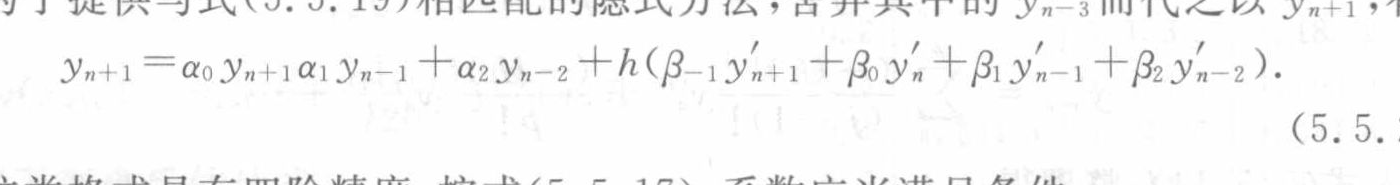
\includegraphics[width=0.85\linewidth,height=\textheight,keepaspectratio,alt={式（5.5.21）原图局部：右端开头的下标与加号排印异常}]{../assets/ch05b/pdf-143-eq521.png}

\href{../../source-images/pdf-144.jpeg}{原页}

\[
y_{n+1}=y_{n-1}+\frac h3(y'_{n+1}+4y'_n+y'_{n-1}).
\tag{5.5.27}
\]

上述格式通常称为 Simpson 格式，用数值积分的 Simpson 方法处理积分恒等式

\[
y(x_{n+1})=y(x_{n-1})+\int_{x_{n-1}}^{x_{n+1}}y'(x)\,\mathrm dx
\]

即可导出这一格式。

用 Simpson 格式（5.5.27）与 Milne 格式（5.5.24）匹配，构成下列预测-校正系统：

预测

\[
\bar y_{n+1}=y_{n-3}+\frac{4h}{3}(2y'_n-y'_{n-1}+2y'_{n-2}),\qquad
\bar y'_{n+1}=f(x_{n+1},\bar y_{n+1});
\]

校正

\[
y_{n+1}=y_{n-1}+\frac h3(\bar y'_{n+1}+4y'_n+y'_{n-1}),\qquad
y'_{n+1}=f(x_{n+1},y_{n+1}).
\]

\subsubsection{5.5.7 Hamming 格式}\label{hamming-ux683cux5f0f}

上述预测-校正系统的缺点是稳定性差。为了改善稳定性，重新挑选校正公式。为此考察式（5.5.21）中不显含 \(y'_{n-2}\) 的一类格式

\[
y_{n+1}=\alpha_0y_n+\alpha_1y_{n-1}+\alpha_2y_{n-2}+h(\beta_{-1}y'_{n+1}+\beta_0y'_n+\beta_1y'_{n-1}),
\tag{5.5.28}
\]

按条件（5.5.22），形如式（5.5.28）的四阶格式含有一个自由度------譬如可取 \(\alpha_1\) 为独立参数。若取 \(\alpha_1=1\) 即得 Simpson 格式（5.5.27）。

Hamming 用 \(\alpha_1\) 的不同数值进行试验，发现当 \(\alpha_1=0\) 时格式的稳定性能较好，即

\[
y_{n+1}=\frac18(9y_n-y_{n-2})+\frac{3h}{8}(y'_{n+1}+2y'_n-y'_{n-1}),
\tag{5.5.29}
\]

其局部截断误差为

\[
y(x_{n+1})-y_{n+1}\approx-\frac{h^5}{40}y_n^{(5)}.
\tag{5.5.30}
\]

Hamming 格式（5.5.29）不能用数值积分方法推导出来。

用 Milne 格式（5.5.24）与 Hamming 格式（5.5.29）相匹配，并利用误差公式（5.5.25）、（5.5.30）改进计算结果，即可建立下列预测-校正系统：

预测

\[
p_{n+1}=y_{n-3}+\frac{4h}{3}(2y'_n-y'_{n-1}+2y'_{n-2}),
\]

改进

\[
m_{n+1}=p_{n+1}-\frac{112}{121}(p_n-c_n),
\]

计算

\[
m'_{n+1}=f(x_{n+1},m_{n+1}),
\]

校正

\[
c_{n+1}=\frac18(9y_n-y_{n-2})+\frac{3h}{8}(m'_{n+1}+2y'_n-y'_{n-1}),
\]

改进

\[
y_{n+1}=c_{n+1}+\frac9{121}(p_{n+1}-c_{n+1}),
\]

\href{../../source-images/pdf-145.jpeg}{原页}

计算

\[
y'_{n+1}=f(x_{n+1},y_{n+1}).
\]

\subsection{5.6 方程组与高阶方程的情形}\label{ux65b9ux7a0bux7ec4ux4e0eux9ad8ux9636ux65b9ux7a0bux7684ux60c5ux5f62}

\subsubsection{5.6.1 一阶方程组}\label{ux4e00ux9636ux65b9ux7a0bux7ec4}

前面研究了单个方程 \(y'=f\) 的数值解法，只要把 \(y\) 和 \(f\) 理解为向量，那么，所提供的各种计算格式即可应用到一阶方程组的情形。

考察一阶方程组

\[
y'_i=f_i(x,y_1,y_2,\cdots,y_N)\qquad(i=1,2,\cdots,N)
\]

的初值问题，初始条件为

\[
y_i(x_0)=y_i^0\qquad(i=1,2,\cdots,N).
\]

若采用向量的记号，记

\[
\boldsymbol y=(y_1,y_2,\cdots,y_N)^{\mathrm T},\qquad
\boldsymbol y^0=(y_1^0,y_2^0,\cdots,y_N^0)^{\mathrm T},
\]

\[
\boldsymbol f=(f_1,f_2,\cdots,f_N)^{\mathrm T},
\]

则上述方程组的初值问题可表示为 \(\begin{cases}\boldsymbol y'=\boldsymbol f(x,\boldsymbol y),\\\boldsymbol y(x_0)=\boldsymbol y_0.\end{cases}\) 求解这一初值问题的四阶 Runge-Kutta 格式为

\[
\boldsymbol y_{n+1}=\boldsymbol y_n+\frac h6(\boldsymbol k_1+2\boldsymbol k_2+2\boldsymbol k_3+\boldsymbol k_4).
\]

其中

\[
\boldsymbol k_1=\boldsymbol f(x_n,\boldsymbol y_n),\qquad
\boldsymbol k_2=\boldsymbol f\left(x_n+\frac h2,\boldsymbol y_n+\frac h2\boldsymbol k_1\right),
\]

\[
\boldsymbol k_3=\boldsymbol f\left(x_n+\frac h2,\boldsymbol y_n+\frac h2\boldsymbol k_2\right),\qquad
\boldsymbol k_4=\boldsymbol f(x_n+h,\boldsymbol y_n+h\boldsymbol k_3);
\]

或表示为

\[
y_{i,n+1}=y_{in}+\frac h6(K_{i1}+2K_{i2}+2K_{i3}+K_{i4})\qquad(i=1,2,\cdots,N),
\]

其中

\[
\begin{aligned}
K_{i1}&=f_i(x_n,y_{1n},y_{2n},\cdots,y_{Nn}),\\
K_{i2}&=f_i\left(x_n+\frac h2,y_{1n}+\frac h2K_{11},y_{2n}+\frac h2K_{21},\cdots,y_{Nn}+\frac h2K_{N1}\right),\\
K_{i3}&=f_i\left(x_n+\frac h2,y_{1n}+\frac h2K_{12},y_{2n}+\frac h2K_{22},\cdots,y_{Nn}+\frac h2K_{N2}\right),\\
K_{i4}&=f_i(x_n+h,y_{1n}+hK_{13},y_{2n}+hK_{23},\cdots,y_{Nn}+hK_{N3}).
\end{aligned}
\]

这里 \(y_{in}\) 是第 \(i\) 个因变量 \(y_i(x)\) 在节点 \(x_n=x_0+nh\) 的近似值。

为了帮助理解这一格式的计算过程，再考察以下两个方程的特殊情形：

\href{../../source-images/pdf-146.jpeg}{原页}

\[
\begin{cases}
y'=f(x,y,z),\quad y(x_0)=y_0,\\
z'=g(x,y,z),\quad z(x_0)=z_0,
\end{cases}
\]

这时四阶 Runge-Kutta 格式具有如下形式：

\[
\begin{cases}
\displaystyle y_{n+1}=y_n+\frac h6(K_1+2K_2+2K_3+K_4),\\[6pt]
\displaystyle z_{n+1}=z_n+\frac h6(L_1+2L_2+2L_3+L_4),
\end{cases}
\tag{5.6.1}
\]

其中

\[
\begin{cases}
K_1=f(x_n,y_n,z_n),\\
\displaystyle K_2=f\left(x_n+\frac h2,y_n+\frac h2K_1,z_n+\frac h2L_1\right),\\[4pt]
\displaystyle K_3=f\left(x_n+\frac h2,y_n+\frac h2K_2,z_n+\frac h2L_2\right),\\[4pt]
K_4=f(x_n+h,y_n+hK_3,z_n+hL_3),\\
L_1=g(x_n,y_n,z_n),\\
\displaystyle L_2=g\left(x_n+\frac h2,y_n+\frac h2K_1,z_n+\frac h2L_1\right),\\[4pt]
\displaystyle L_3=g\left(x_n+\frac h2,y_n+\frac h2K_2,z_n+\frac h2L_2\right),\\[4pt]
L_4=g(x_n+h,y_n+hK_3,z_n+hL_3).
\end{cases}
\tag{5.6.2}
\]

这是一步法，利用节点 \(x_n\) 上的值 \(y_n,z_n\)，由式（5.6.2）顺序计算 \(K_1,\allowbreak L_1,\allowbreak K_2,\allowbreak L_2,\allowbreak K_3,\allowbreak L_3,\allowbreak K_4,\allowbreak L_4\)，然后代入式（5.6.1）即可求得节点 \(x_{n+1}\) 上的 \(y_{n+1},z_{n+1}\)。

\subsubsection{5.6.2 化高阶方程组为一阶方程组}\label{ux5316ux9ad8ux9636ux65b9ux7a0bux7ec4ux4e3aux4e00ux9636ux65b9ux7a0bux7ec4}

关于高阶微分方程（或方程组）的初值问题，原则上总可以归结为一阶方程组来求解。例如，考察下列 \(m\) 阶微分方程：

\[
y^{(m)}=f(x,y,y',\cdots,y^{(m-1)}),
\tag{5.6.3}
\]

初始条件为

\[
y(x_0)=y_0,\quad y'(x_0)=y'_0,\quad\cdots,\quad y^{(m-1)}(x_0)=y_0^{(m-1)}.
\tag{5.6.4}
\]

只要引进新的变量 \(y_1=y,y_2=y',\cdots,y_m=y^{(m-1)}\)，即可将 \(m\) 阶方程（5.6.3）化为如下的一阶方程组：

\[
\begin{cases}
y'_1=y_2,\\
y'_2=y_3,\\
\qquad\vdots\\
y'_{m-1}=y_m,\\
y'_m=f(x,y_1,y_2,\cdots,y_m);
\end{cases}
\tag{5.6.5}
\]

初始条件（5.6.4）则相应地化为

\href{../../source-images/pdf-147.jpeg}{原页}

\[
y_1(x_0)=y_0,\quad y_2(x_0)=y'_0,\quad\cdots,\quad y_m(x_0)=y_0^{(m-1)}.
\tag{5.6.6}
\]

不难证明，初值问题（5.6.3）、（5.6.4）和（5.6.5）、（5.6.6）是彼此等价的。

特别地，对于下列二阶方程的初值问题：

\[
\begin{cases}
y''=f(x,y,y'),\\
y(x_0)=y_0,\quad y'(x_0)=y'_0.
\end{cases}
\]

引进新的变量 \(z=y'\)，即可化为下列一阶方程组的初值问题：

\[
\begin{cases}
y'=z,\quad y(x_0)=y_0,\\
z'=f(x,y,z),\quad z(x_0)=y'_0.
\end{cases}
\]

针对这个问题应用四阶 Runge-Kutta 格式（5.6.1），有

\[
\begin{cases}
\displaystyle y_{n+1}=y_n+\frac h6(K_1+2K_2+2K_3+K_4),\\[6pt]
\displaystyle z_{n+1}=z_n+\frac h6(L_1+2L_2+2L_3+L_4).
\end{cases}
\]

按式（5.6.2），有

\[
K_1=z_n,\quad L_1=f(x_n,y_n,z_n);
\]

\[
K_2=z_n+\frac h2L_1,\quad
L_2=f\left(x_n+\frac h2,y_n+\frac h2K_1,z_n+\frac h2L_1\right);
\]

\[
K_3=z_n+\frac h2L_2,\quad
L_3=f\left(x_n+\frac h2,y_n+\frac h2K_2,z_n+\frac h2L_2\right);
\]

\[
K_4=z_n+hL_3,\quad L_4=f(x_n+h,y_n+hK_3,z_n+hL_3).
\]

如果消去 \(K_1,K_2,K_3,K_4\)，则上述格式可表示为

\[
\begin{cases}
\displaystyle y_{n+1}=y_n+hz_n+\frac{h^2}{6}(L_1+L_2+L_3),\\[6pt]
\displaystyle z_{n+1}=z_n+\frac h6(L_1+2L_2+2L_3+L_4),
\end{cases}
\]

这里

\[
L_1=f(x_n,y_n,z_n),
\]

\[
L_2=f\left(x_n+\frac h2,y_n+\frac h2z_n,z_n+\frac h2L_1\right),
\]

\[
L_3=f\left(x_n+\frac h2,y_n+\frac h2z_n+\frac{h^2}{4}L_1,z_n+\frac h2L_2\right),
\]

\[
L_4=f\left(x_n+h,y_n+hz_n+\frac{h^2}{2}L_2,z_n+hL_3\right).
\]

\subsection{5.7 边值问题的数值解法}\label{ux8fb9ux503cux95eeux9898ux7684ux6570ux503cux89e3ux6cd5}

在具体求解微分方程时，必须附加某种定解条件。微分方程和定解条件一起组成定

\href{../../source-images/pdf-148.jpeg}{原页}

（接上页）解问题。对于高阶微分方程，定解条件通常有两种给法：一种是给出了积分曲线在初始时刻的性态，这类条件称为\textbf{初始条件}，相应的定解问题称为\textbf{初值问题}；另一种是给出了积分曲线首末两端的性态，这类条件则称为\textbf{边界条件}，相应的定解问题称为\textbf{边值问题}。

以二阶方程

\[
y''=f(x,y,y')
\tag{5.7.1}
\]

为例，其初始条件的给法是

\[
y(a)=\alpha,\quad y'(a)=m.
\tag{5.7.2}
\]

前面已经研究过这种初值问题的数值解法。

设在区间 \(a<x<b\) 上求解方程（5.7.1），则边界条件可以给为

\[
y(a)=\alpha,\quad y(b)=\beta.
\tag{5.7.3}
\]

\subsubsection{5.7.1 试射法}\label{ux8bd5ux5c04ux6cd5}

可以用所谓``试射法''来求解边值问题（5.7.1）、（5.7.3）。这种方法的基本思想是设法将边值问题转化为初值问题来求解，即依据边界条件（5.7.3）寻求与它等价的初始条件（5.7.2），也就是说，反复调整初始时刻的斜率值 \(y'(a)=m\)，使初值问题（5.7.1）、（5.7.2）的积分曲线 \(y=y(x)\) 能``命中''\(y(b)=\beta\)（见图 5.5）。

试射法的计算过程很简单。设凭经验能够提供 \(m\) 的两个预测值 \(m_1,m_2\)，分别按这两个斜率值``试射''------求解相应的初值问题（5.7.1）、（5.7.2），从而获得 \(y(b)\) 的两个结果 \(\beta_1,\beta_2\)。如果 \(\beta_1\) 与 \(\beta_2\) 均不满足预定的精度，就用线性插值方法校正 \(m_1,m_2\) 得新的斜率值

\[
m_3=m_1+\frac{m_2-m_1}{\beta_2-\beta_1}(\beta-\beta_1),
\]

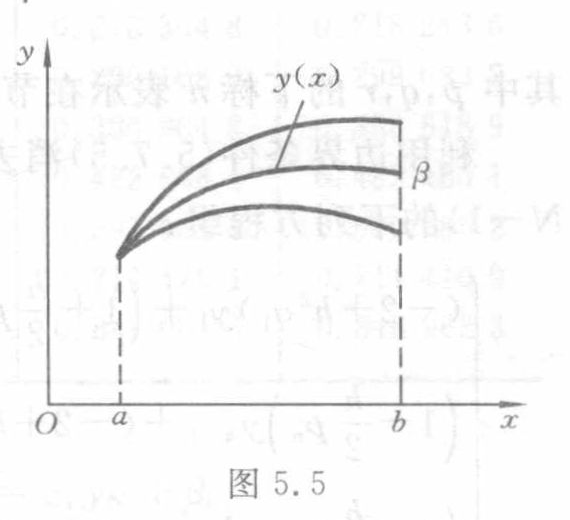
\includegraphics[width=0.85\linewidth,height=\textheight,keepaspectratio,alt={图 5.5（原图）试射法示意}]{../assets/ch05b/figure-5-5.png}

图 5.5（原图）符号与图意：坐标轴 \(x,y\)，原点 \(O\)，横轴端点 \(a,b\)，目标右端值 \(\beta\)，积分曲线标记 \(y(x)\)。三条曲线从 \(x=a\) 的同一左端点出发，在 \(x=b\) 处到达不同高度；\(y(x)\) 指向达到目标 \(\beta\) 的中间曲线。端点位置以竖虚线标出；图中未给出具体函数或数值。

然后再按斜率值 \(m_3\) 试射，求解相应的初值问题（5.7.1）、（5.7.2），又得新的结果 \(y(b)=\beta_3\)。继续这一过程，直到计算结果 \(y(b)\) 与 \(\beta\) 相当符合为止。

上述试射法过分依赖于经验，局限性大。下面介绍求解边值问题的差分方法。

\subsubsection{5.7.2 差分方程的建立}\label{ux5deeux5206ux65b9ux7a0bux7684ux5efaux7acb}

应用差分方法的关键，在于恰当地选取差商逼近微分方程中的导数。我们知道，逼近一阶导数 \(y'(x)\) 可用向前差商 \(\dfrac{y(x+h)-y(x)}h\)，亦可用向后差商 \(\dfrac{y(x)-y(x-h)}h\) 或中心差商 \(\dfrac{y(x+h)-y(x-h)}{2h}\)。中心差商是向前差商与向后差商的算术平均。为逼近二阶导数 \(y''(x)\)，一般用二阶差商------向前差商的向后差商（即向后差商的向前差商）

\href{../../source-images/pdf-149.jpeg}{原页}

\[
y''(x)\approx\frac{\dfrac{y(x+h)-y(x)}h-\dfrac{y(x)-y(x-h)}h}{h}
=\frac{y(x+h)-2y(x)+y(x-h)}{h^2}.
\]

设将积分区间 \([a,b]\) 划分为 \(N\) 等份，步长 \(h=\dfrac{b-a}{N}\)，节点 \(x_n=x_0+nh,n=0,1,\cdots,N\)。用差商替代相应的导数，可将边值问题（5.7.1）、（5.7.3）离散化得下列计算公式：

\[
\frac{y_{n+1}-2y_n+y_{n-1}}{h^2}=f\left(x_n,y_n,\frac{y_{n+1}-y_{n-1}}{2h}\right)\qquad(n=1,2,\cdots,N-1),
\tag{5.7.4}
\]

\[
y_0=\alpha,\quad y_N=\beta.
\tag{5.7.5}
\]

如果函数 \(f\) 是非线性的，那么所归结出的差分方程也是非线性的，这时实际求解比较困难。

如果所给方程（5.7.1）是如下形式的线性方程：

\[
y''+p(x)y'+q(x)y=r(x),
\tag{5.7.6}
\]

则差分方程（5.7.4）相应的形式为

\[
\frac{y_{n+1}-2y_n+y_{n-1}}{h^2}+p_n\frac{y_{n+1}-y_{n-1}}{2h}+q_ny_n=r_n\qquad(n=1,\cdots,N-1),
\tag{5.7.7}
\]

其中 \(p,q,r\) 的下标 \(n\) 表示在节点 \(x_n\) 取值。

利用边界条件（5.7.5）消去式（5.7.7）中的 \(y_0\) 和 \(y_N\)，整理得到关于 \(y_n\)（\(1\le n\le N-1\)）的下列方程组：

\[
\begin{cases}
\displaystyle(-2+h^2q_1)y_1+\left(1+\frac h2p_1\right)y_2=h^2r_1-\left(1-\frac h2p_1\right)\alpha,\\[6pt]
\displaystyle\left(1-\frac h2p_n\right)y_{n-1}+(-2+h^2q_n)y_n+\left(1+\frac h2p_n\right)y_{n+1}=h^2r_n\quad(2\le n\le N-2),\\[6pt]
\displaystyle\left(1-\frac h2p_{N-1}\right)y_{N-2}+(-2+h^2q_{N-1})y_{N-1}=h^2r_{N-1}-\left(1+\frac h2p_{N-1}\right)\beta.
\end{cases}
\tag{5.7.8}
\]

这样归结出的方程组是所谓\textbf{三对角型}的，即

\[
\begin{pmatrix}
-2+h^2q_1 & 1+\dfrac h2p_1 & & & \\
1-\dfrac h2p_2 & -2+h^2q_2 & 1+\dfrac h2p_2 & & \\
& \ddots & \ddots & \ddots & \\
& & 1-\dfrac h2p_{N-2} & -2+h^2q_{N-2} & 1+\dfrac h2p_{N-2} \\
& & & 1-\dfrac h2p_{N-1} & -2+h^2q_{N-1}
\end{pmatrix},
\]

\href{../../source-images/pdf-150.jpeg}{原页}

因为它的系数矩阵仅在主对角线及其相邻的两条对角线上有非零元素。求解这种三对角型方程组，用所谓\textbf{追赶法}特别有效。在 7.4.3 节将介绍追赶法。

\textbf{例 5.7} 用差分方法解边值问题 \(\begin{cases}y''-y=x,\quad0<x<1,\\y(0)=0,\quad y(1)=1.\end{cases}\)

\textbf{解} 取步长 \(h=0.1\)，节点 \(x_n=\dfrac n{10}\)（\(n=0,1,2,\cdots,10\)），差分方程（5.7.8）的形式是

\[
\begin{pmatrix}
-2-10^{-2}&1&&&\\
1&-2-10^{-2}&1&&\\
&\ddots&\ddots&\ddots&\\
&&1&-2-10^{-2}&1\\
&&&1&-2-10^{-2}
\end{pmatrix}
\begin{pmatrix}y_1\\y_2\\\vdots\\y_8\\y_9\end{pmatrix}
=
\begin{pmatrix}0.1\times10^{-2}\\0.2\times10^{-2}\\\vdots\\0.8\times10^{-2}\\-1+0.9\times10^{-2}\end{pmatrix}.
\]

表 5.11 列出了差分方法的计算结果，表中最末一列是按解的表达式

\[
y=\frac{2(\mathrm e^x-\mathrm e^{-x})}{\mathrm e-\mathrm e^{-1}}-x
\]

算出的准确值。

\textbf{表 5.11}

{\def\LTcaptype{none} % do not increment counter
\begin{longtable}[]{@{}lrr@{}}
\toprule\noalign{}
\(x_n\) & \(y_n\) & \(y(x_n)\) \\
\midrule\noalign{}
\endhead
\bottomrule\noalign{}
\endlastfoot
0.1 & 0.0704894 & 0.0704673 \\
0.2 & 0.1426836 & 0.1426409 \\
0.3 & 0.2183048 & 0.2182436 \\
0.4 & 0.2991089 & 0.2990332 \\
0.5 & 0.3869042 & 0.3868189 \\
0.6 & 0.4835684 & 0.4834801 \\
0.7 & 0.5910684 & 0.5909852 \\
0.8 & 0.7114791 & 0.7114109 \\
0.9 & 0.8470045 & 0.8469633 \\
\end{longtable}
}

附带指出，在应用上，有时边界条件按以下方式给出：

当 \(x=a\) 时，\(y'=\alpha_0y+\beta_0\)；当 \(x=b\) 时，\(y'=\alpha_1y+\beta_1\)。

这里 \(\alpha_0,\beta_0,\alpha_1,\beta_1\) 均为已知常数，这时，边界条件中所包含的微商也要替换成相应的差商

\[
\frac{y_1-y_0}{h}=\alpha_0y_0+\beta_0,\qquad
\frac{y_N-y_{N-1}}h=\alpha_1y_N+\beta_1.
\]

它们和差分方程（5.7.7）一起，仍然构成包含 \(N+1\) 个未知数的线性方程组。

\subsubsection{5.7.3 差分问题的可解性}\label{ux5deeux5206ux95eeux9898ux7684ux53efux89e3ux6027}

我们知道，通过自变量的适当变换可以消除线性方程（5.7.6）中的一阶导数项。下面仅就缺一阶导数项的方程来讨论这一问题。考察边值问题

\[
\begin{cases}
y''-q(x)y=r(x),\\
y(a)=\alpha,\quad y(b)=\beta.
\end{cases}
\tag{5.7.9}
\]

这里假定 \(q(x)\ge0\)，其对应的差分问题是

\[
\begin{cases}
\displaystyle\frac{y_{n+1}-2y_n+y_{n-1}}{h^2}-q_ny_n=r_n\quad(n=1,2,\cdots,N-1),\\[6pt]
y_0=\alpha,\quad y_N=\beta.
\end{cases}
\tag{5.7.10}
\]

\href{../../source-images/pdf-151.jpeg}{原页}

现在论证差分问题的可解性。由于式（5.7.10）是关于变量 \(y_n\)（\(n=0,1,2,\cdots,N\)）的线性方程组，要证明它的解存在唯一，只要证明对应的齐次方程组只有零解。为此，我们引进下述极值原理。

\textbf{定理 5.2} 对于一组不全相等的数 \(y_n\)（\(n=0,1,\cdots,N\)），记

\[
l(y_n)=\frac{y_{n+1}-2y_n+y_{n-1}}{h^2}-q_ny_n,\quad q_n\ge0\qquad(n=1,2,\cdots,N-1).
\]

假定 \(l(y_n)\ge0\)（\(n=1,2,\cdots,N-1\)），则 \(y_n\) 的正的最大值只能是 \(y_0\) 或 \(y_N\)；如果 \(l(y_n)<0\)（\(n=1,2,\cdots,N-1\)），则 \(y_n\) 的负的最小值只能是 \(y_0\) 或 \(y_N\)。

\textbf{证明} 用反证法。考察 \(l(y_n)\ge0\) 的情形，设 \(y_m\)（\(0<m<N\)）是正的最大值，即 \(y_m=\max_{0\le n\le N}y_n=M>0\)，且 \(y_{m-1}\) 和 \(y_{m+1}\) 中至少有一个小于 \(M\)，此时有

\[
l(y_m)=\frac{y_{m+1}-2y_m+y_{m-1}}{h^2}-q_my_m<\frac{M-2M+M}{h^2}-q_mM=-q_mM,
\]

由于 \(q_m\ge0,M>0\)，故由上式推出 \(l(y_m)<0\)，此与题设矛盾。

此外，\(l(y_n)<0\) 的情形可类似地进行讨论。证毕。

作为这一定理的推论有如下定理。

\textbf{定理 5.3} 差分问题式（5.7.10）的解存在并且是唯一的。

\textbf{证明} 只要证明对应的齐次方程组

\[
\begin{cases}
\displaystyle l(y_n)=\frac{y_{n+1}-2y_n+y_{n-1}}{h^2}-q_ny_n=0\quad(n=1,2,\cdots,N-1),\\[6pt]
y_0=y_N=0
\end{cases}
\]

只有零解。由于这里 \(l(y_n)=0\)（\(n=1,2,\cdots,N-1\)），由极值原理知，\(y_n\) 的正的最大值和负的最小值只能是 \(y_0\) 或 \(y_N\)，而按边界条件 \(y_0=y_N=0\)，故所有的 \(y_n\)（\(n=0,1,\cdots,N\)）全为零。证毕。

\subsubsection{5.7.4 差分方法的收敛性}\label{ux5deeux5206ux65b9ux6cd5ux7684ux6536ux655bux6027}

现在运用极值原理论证差分方法的收敛性并估计误差。

\textbf{定理 5.4} 设 \(y_n\) 是差分问题式（5.7.10）的解，而 \(y(x_n)\) 是边值问题（5.7.9）的解 \(y(x)\) 在节点 \(x_n\) 的值，则截断误差 \(e_n=y(x_n)-y_n\) 有下列估计式：

\[
|e_n|\le\frac{M(b-a)^2}{96}h^2,\qquad
M=\max_{a\le x\le b}|y^{(4)}(x)|.
\tag{5.7.11}
\]

\textbf{证明} 由 Taylor 展开，易得

\[
\begin{cases}
\displaystyle\frac{y(x_{n+1})-2y(x_n)+y(x_{n-1})}{h^2}-q_ny(x_n)=r_n+\frac{h^2}{12}y^{(4)}(\xi_n),\quad x_{n-1}<\xi_n<x_{n+1},\\[6pt]
y(x_0)=\alpha,\quad y(x_N)=\beta.
\end{cases}
\tag{5.7.12}
\]

\begin{quote}
校注（agent 补充）：定理 5.2 的负最小值一侧，原书确实写作严格条件 \(l(y_n)<0\)；定理 5.3 却在 \(l(y_n)=0\) 时同时引用正最大值、负最小值结论。此处原文均照录。补足该引用的方法是对 \(-y_n\) 应用定理 5.2 的 \(l\ge0\) 一侧（利用 \(l\) 的线性），从而排除负最小值；无需改动原书方程。
\end{quote}

\href{../../source-images/pdf-152.jpeg}{原页}

将式（5.7.12）与式（5.7.10）相减，知截断误差 \(e_n=y(x_n)-y_n\) 满足

\[
\begin{cases}
\displaystyle l(e_n)=\frac{e_{n+1}-2e_n+e_{n-1}}{h^2}-q_ne_n=\frac{h^2}{12}y^{(4)}(\xi_n),\\[6pt]
e_0=e_N=0,
\end{cases}
\]

其中 \(\xi_n\) 一般是不知道的。于是转向下列差分问题：

\[
\begin{cases}
\displaystyle l(\varepsilon_n)=\frac{\varepsilon_{n+1}-2\varepsilon_n+\varepsilon_{n-1}}{h^2}-q_n\varepsilon_n=-\frac{h^2}{12}M,\\[6pt]
\varepsilon_0=\varepsilon_N=0,
\end{cases}
\tag{5.7.13}
\]

其中 \(M=\max_{a\le x\le b}|y^{(4)}(x)|\)。首先证明上述两个差分问题的解存在下列关系：

\[
|e_n|\le\varepsilon_n\qquad(n=0,1,\cdots,N).
\tag{5.7.14}
\]

事实上，由于

\[
l(\varepsilon_n)=-\frac{h^2}{12}M\le-\frac{h^2}{12}|y^{(4)}(\xi_n)|=-|l(e_n)|,
\]

故有

\[
l(\varepsilon_n-e_n)\le0,\qquad l(\varepsilon_n+e_n)\le0.
\]

又

\[
\varepsilon_0-e_0=\varepsilon_N-e_N=0,\qquad\varepsilon_0+e_0=\varepsilon_N+e_N=0,
\]

利用定理 5.2，知 \(\varepsilon_n-e_n\ge0,\varepsilon_n+e_n\ge0\)，即式（5.7.14）成立。

差分问题（5.7.13）的解仍不易直接求得，于是进一步考察

\[
\begin{cases}
\displaystyle\tilde l(\rho_n)=\frac{\rho_{n+1}-2\rho_n+\rho_{n-1}}{h^2}=-\frac{h^2}{12}M,\\[6pt]
\rho_0=\rho_N=0.
\end{cases}
\tag{5.7.15}
\]

这里 \(\tilde l(\rho_n-\varepsilon_n)=-q_n\varepsilon_n\le0\)，又 \(\rho_0-\varepsilon_0=\rho_N-\varepsilon_N=0\)，故由定理 5.2（注意，当 \(q_n=0\) 时，\(l(\tilde y_n)\) 就是 \(l(y_n)\)）知 \(\rho_n-\varepsilon_n\ge0\)，即 \(\varepsilon_n\le\rho_n\)，于是有 \(|e_n|\le\varepsilon_n\le\rho_n\)。

然而 \(\rho_n\) 是容易求出的。求解差分问题（5.7.15）所对应的边值问题

\[
\begin{cases}
\displaystyle\rho''=-\frac{h^2}{12}M,\\[6pt]
\rho(a)=\rho(b)=0,
\end{cases}
\]

解得

\[
\rho(x)=\frac{h^2}{24}M(x-a)(b-x).
\]

容易验证 \(\rho_n=\rho(x_n)\) 是差分问题（5.7.15）的解，注意到 \(\rho(x)\) 在点 \(x=\dfrac{a+b}2\) 达到最大值

\[
\rho\left(\frac{a+b}2\right)=\frac{M(b-a)^2}{96}h^2,
\]

因此有估计式（5.7.11）。证毕。

据估计式（5.7.11）知，当 \(h\to0\) 时有 \(e_n\to0\)，这表明差分方法（5.7.10）是收敛的。

\begin{quote}
校注（agent 补充，ch05b-E006）：式（5.7.15）后括注的原图在 \(y\) 上方印波浪号，即 \(l(\tilde y_n)\)，这里照录。按该式定义与``当 \(q_n=0\) 时''的上下文，此处疑将波浪号排错位置，预期为 \(\tilde l(y_n)\)，即去掉零阶项后的算子；原文并未定义 \(\tilde y_n\)。
\end{quote}

\href{../../source-images/pdf-153.jpeg}{原页}

\subsection{小结}\label{ux5c0fux7ed3}

本章研究求解常微分方程的差分方法。构造差分格式主要有两条途径：基于数值积分的构造方法和基于 Taylor 展开的构造方法。后一种方法更灵活，也更具有一般性。Taylor 展开方法还有一个优点，它在构造差分公式的同时可以得到关于截断误差的估计。

但是，直接用 Taylor 展开导出的 Taylor 级数法（见 7.3.1 节）不便于实际应用。基于 Taylor 展开构造出的四阶 Runge-Kutta 方法（见 7.3.4 节）则是电子计算机上的常用算法。四阶 Runge-Kutta 方法的优点是精度高，程序简单，计算过程稳定，并且易于调节步长。

四阶 Runge-Kutta 方法也有不足之处，它要求函数 \(f\) 具有较高的光滑性。如果 \(f\) 的光滑性差，那么它的精度可能还不如 Euler 格式（见 7.2.1 节）或改进的 Euler 格式（见 7.2.4 节）。

四阶 Runge-Kutta 方法的另一个缺点是计算量比较大，需要耗费较多的机器时间（每一步需四次计算函数 \(f\) 的值）。相比之下，Hamming 方法（见 7.5.7 节）可以节省计算量（每一步只需两次计算函数 \(f\) 的值）。但 Hamming 方法是一种四步法，它不是自开始的，需要借助于四阶 Runge-Kutta 方法（或四阶 Taylor 级数法）提供开始值。

就差分方法来说，常微分方程与偏微分方程有着紧密的联系，读者可参看偏微分方程的数值解法的有关教材。

\subsection{习题}\label{ux4e60ux9898}

\begin{enumerate}
\def\labelenumi{\arabic{enumi}.}
\item
  就初值问题 \(y'=ax+b,y(0)=0\) 分别导出 Euler 方法和改进的 Euler 方法的近似解的表达式，并与准确解 \(y=\dfrac12ax^2+bx\) 相比较。
\item
  用改进的 Euler 方法解初值问题 \(\begin{cases}y'=x+y,\quad0<x<1,\\y(0)=1,\end{cases}\) 取步长 \(h=0.1\) 计算，并与准确解 \(y=-x-1+2\mathrm e^x\) 相比较。
\item
  用改进的 Euler 方法解 \(\begin{cases}y'=x^2+x-y,\\y(0)=0,\end{cases}\) 取步长 \(h=0.1\) 计算 \(y(0.5)\)，并与准确解 \(y=-\mathrm e^{-x}+x^2-x+1\) 相比较。
\item
  用梯形方法解初值问题 \(\begin{cases}y'+y=0,\\y(0)=1,\end{cases}\) 证明其近似解为 \(y_n=\left(\dfrac{2-h}{2+h}\right)^n\)，并证明当 \(h\to0\) 时，它收敛于原初值问题的准确解 \(y=\mathrm e^{-x}\)。
\item
  利用 Euler 方法计算积分 \(\displaystyle\int_0^x\mathrm e^{t^2}\,\mathrm dt\) 在点 \(x=0.5,1,1.5,2\) 的近似值。
\end{enumerate}

\begin{quote}
校注（agent 补充，ch05b-E007）：小结中的五处节号按原印刷保留为 7.3.1、7.3.4、7.2.1、7.2.4、7.5.7；这些节号与本版章节编排不符。对应主题在本书章节索引中分别为 5.3.1（Taylor 级数法）、5.3.5（四阶 Runge-Kutta 方法）、5.2.1（Euler 格式）、5.2.4（改进的 Euler 格式）、5.5.7（Hamming 格式）。其中本章 PDF 140 的正文也明确将四阶 Runge-Kutta 格式指向 5.3.5，PDF 144 的实际标题为 5.5.7 Hamming 格式。
\end{quote}

\href{../../source-images/pdf-154.jpeg}{原页}

\textbf{6.} 取 \(h=0.2\)，用经典的四阶 Runge-Kutta 方法求解下列初值问题：

（1）\(\begin{cases}y'=x+y,\quad0<x<1,\\y(0)=1;\end{cases}\)

（2）\(\begin{cases}y'=3y/(1+x),\quad0<x<1,\\y(0)=1.\end{cases}\)

\textbf{7.} 证明对任意参数 \(t\)，下列 Runge-Kutta 格式是二阶的：

\[
\begin{cases}
\displaystyle y_{n+1}=y_n+\frac h2(K_2+K_3),\\[6pt]
K_1=f(x_n,y_n),\\
K_2=f(x_n+th,y_n+thK_1),\\
K_3=f(x_n+(1-t)h,y_n+(1-t)hK_1).
\end{cases}
\]

\textbf{8.} 证明下列两种 Runge-Kutta 方法是三阶的：

（1）

\[
\begin{cases}
\displaystyle y_{n+1}=y_n+\frac h4(K_1+3K_3),\\[6pt]
K_1=f(x_n,y_n),\\
\displaystyle K_2=f\left(x_n+\frac h3,y_n+\frac h3K_1\right),\\[4pt]
\displaystyle K_3=f\left(x_n+\frac23h,y_n+\frac23hK_2\right);
\end{cases}
\]

（2）

\[
\begin{cases}
\displaystyle y_{n+1}=y_n+\frac h9(2K_1+3K_2+4K_3),\\[6pt]
K_1=f(x_n,y_n),\\
\displaystyle K_2=f\left(x_n+\frac h2,y_n+\frac h2K_1\right),\\[4pt]
\displaystyle K_3=f\left(x_n+\frac34h,y_n+\frac34hK_2\right).
\end{cases}
\]

\textbf{9.} 分别用二阶显式 Adams 方法和二阶隐式 Adams 方法解下列初值问题：

\[
y'=1-y,\quad y(0)=0,
\]

取 \(h=0.2,y_0=0,y_1=0.181\)，计算 \(y(1.0)\) 并与准确解 \(y=1-\mathrm e^{-x}\) 相比较。

\textbf{10.} 证明下列解 \(y'=f(x,y)\) 的差分公式

\[
y_{n+1}=\frac12(y_n+y_{n-1})+\frac h4(4y'_{n+1}-y'_n+3y'_{n-1})
\]

是二阶的，并求出截断误差的首项。

\textbf{11.} 导出具有下列形式的三阶方法：

\[
y_{n+1}=a_0y_n+a_1y_{n-1}+a_2y_{n-2}+h(b_0y'_n+b_1y'_{n-1}+b_2y'_{n-2}).
\]

\textbf{12.} 将下列方程化为一阶方程组：

（1）\(y''-3y'+2y=0,\quad y(0)=1,\quad y'(0)=1\)；

（2）\(y''-0.1(1-y^2)y'+y=0,\quad y(0)=1,\quad y'(0)=0\)；

（3）\(x''(t)=-\dfrac{x}{r^3},\allowbreak \quad y''(t)=-\dfrac{y}{r^3},\allowbreak \quad r=\sqrt{x^2+y^2},\allowbreak \quad x(0)=0.4,\allowbreak \quad x'(0)=0,\allowbreak \quad y(0)=0,\allowbreak \quad y'(0)=2\)。

\textbf{13.} 取 \(h=0.25\)，用差分法解边值问题 \(\begin{cases}y''+y=0,\\y(0)=0,\quad y(1)=1.68.\end{cases}\)

\textbf{14.} 对方程 \(y''=f(x,y)\) 可建立差分公式 \(y_{n+1}=2y_n-y_{n-1}+h^2f(x_n,y_n)\)，试用这一公式求解初值问题 \(\begin{cases}y''=1,\\y(0)=y(1)=0,\end{cases}\) 验证计算解恒等于准确解 \(y(x)=\dfrac{x^2-x}{2}\)。

\textbf{15.} 取 \(h=0.2\)，用差分方法解边值问题 \(\begin{cases}(1+x^2)y''-xy'-3y=6x-3,\\y(0)-y'(0)=1,\quad y(1)=2.\end{cases}\)

\begin{quote}
校注（agent 补充，ch05b-E008）：习题 14 原书写``初值问题''，已照录；但给定条件为两端的 \(y(0)=y(1)=0\)，按本章定义属于边值问题，疑为称谓误植。此处只标记原书疑误，未代做习题。
\end{quote}

\subsection{本节覆盖原页的校注记录}\label{ux672cux8282ux8986ux76d6ux539fux9875ux7684ux6821ux6ce8ux8bb0ux5f55}

下列记录按原页关联，含同页相邻小节的校注；计算时同时读取上文校注和完整原页。

\begin{itemize}
\tightlist
\item
  \texttt{ch05a-E001}：原书 PDF 页 124
\item
  \texttt{ch05a-E002}：原书 PDF 页 124
\item
  \texttt{ch05a-E003}：原书 PDF 页 129
\item
  \texttt{ch05a-E004}：原书 PDF 页 134
\item
  \texttt{ch05a-E005}：原书 PDF 页 134
\item
  \texttt{ch05a-E006}：原书 PDF 页 135
\item
  \texttt{ch05a-E007}：原书 PDF 页 136
\item
  \texttt{ch05b-E001}：原书 PDF 页 138
\item
  \texttt{ch05b-E002}：原书 PDF 页 141
\item
  \texttt{ch05b-E003}：原书 PDF 页 141
\item
  \texttt{ch05b-E004}：原书 PDF 页 141
\item
  \texttt{ch05b-E005}：原书 PDF 页 143
\item
  \texttt{ch05b-E006}：原书 PDF 页 152
\item
  \texttt{ch05b-E007}：原书 PDF 页 153
\item
  \texttt{ch05b-E008}：原书 PDF 页 154
\end{itemize}

\end{document}
